\documentclass{tufte-book}

\hypersetup{colorlinks}

\title[PETSc for PDEs]{PETSc \\ for \\ Partial \\ Differential \\ Equations}
\author{Ed Bueler}
\publisher{Maybe Someday a Publisher of This Book}

\date{\today}

\usepackage{booktabs} % for nicely-typeset tabular material
\usepackage{verbatim} % for "comment" environment
\usepackage{xspace}
\usepackage{fancyvrb}
\usepackage{graphicx}
\usepackage{amsmath,amssymb,amsthm,bm}
\usepackage{tikz}
\usetikzlibrary{arrows,decorations.markings}

\usepackage[subtle,floats]{savetrees}

% macros

\theoremstyle{definition}
\newtheorem*{example}{{\color{cyan} Example}}

\newcommand{\trueinput}[2]{
\VerbatimInput[frame=single,framesep=3mm,label=\fbox{\normalsize \textsl{\,#1\,}},fontfamily=courier,fontsize=\footnotesize]{#2}
}

%\inputfromline{FULLPATH}{FILENAME}{CAPTION}{FIRSTLINE}{LABEL}
\newcommand{\inputfromline}[5]{
\vspace{0.8cm}
\let\FancyVerbStartString\relax
\let\FancyVerbStopString\relax
\begin{minipage}[l]{1.25\textwidth}
\VerbatimInput[frame=single,%
               framesep=3mm,%
               label=\fbox{\small \textsl{\,#2\,}},%
               fontfamily=courier,%
               fontsize=\scriptsize,%
               firstline=#4]{#1}
\end{minipage}
\vspace{0.5cm}

\begin{marginfigure}[1.0cm]
\caption{#3}
\label{#5}
\end{marginfigure}

\vspace{1.5cm}
}

\newcommand{\inputwhole}[4]{\inputfromline{#1}{#2}{#3}{1}{#4}}

%\cinputraw{FULLPATH}{FILENAME}{CAPTION}{PARTSTRING}{STARTSTRING}{STOPSTRING}{LABEL}
\newcommand{\cinputraw}[7]{
\newcommand*\FancyVerbStartString{#5}
\newcommand*\FancyVerbStopString{#6}
\vspace{0.8cm}
\begin{minipage}[l]{1.25\textwidth}
\VerbatimInput[frame=single,%
               framesep=3mm,%
               label=\fbox{\small \textsl{\,#2\,}#4},%
               fontfamily=courier,%
               fontsize=\scriptsize]{#1}
\end{minipage}
\vspace{0.5cm}

\begin{marginfigure}[1.0cm]
\caption{#3}
\label{#7}
\end{marginfigure}

\vspace{1.5cm}
\let\FancyVerbStartString\relax
\let\FancyVerbStopString\relax
}

\newcommand{\cinput}[5]{%
    \cinputraw{cstrip/#1}{#1}{#2}{}{#3}{#4}{#5}}
\newcommand{\cinputnostrip}[5]{%
    \cinputraw{../c/#1}{#1}{#2}{}{#3}{#4}{#5}}

\newcommand{\cinputpart}[6]{%
    \cinputraw{cstrip/#1}{#1}{#2}{\quad \textbf{part #3}}{#4}{#5}{#6}}
\newcommand{\cinputpartnostrip}[6]{%
    \cinputraw{../c/#1}{#1}{#2}{\quad \textbf{part #3}}{#4}{#5}{#6}}

\newcommand{\caveat}[1]{\marginnote{\textsc{Where we stand:}\\  #1}}

% Prints an epigraph and speaker in sans serif, all-caps type.
\newcommand{\openepigraph}[2]{%
  %\sffamily\fontsize{14}{16}\selectfont
  \begin{fullwidth}
  \sffamily\large
  \begin{doublespace}
  \noindent\allcaps{#1}\\% epigraph
  \noindent \Large \allcaps{#2}% author
  \end{doublespace}
  \end{fullwidth}
}

\newcommand{\monthyear}{%
  \ifcase\month\or January\or February\or March\or April\or May\or June\or
  July\or August\or September\or October\or November\or
  December\fi\space\number\year
}

\newcommand{\bA}{\mathbf{A}}
\newcommand{\bB}{\mathbf{B}}
\newcommand{\bE}{\mathbf{E}}
\newcommand{\bF}{\mathbf{F}}
\newcommand{\bJ}{\mathbf{J}}

\newcommand{\bb}{\mathbf{b}}
\newcommand{\bn}{\mathbf{n}}
\newcommand{\br}{\mathbf{r}}
\newcommand{\bu}{\mathbf{u}}
\newcommand{\bv}{\mathbf{v}}
\newcommand{\bw}{\mathbf{w}}
\newcommand{\bx}{\mathbf{x}}
\newcommand{\by}{\mathbf{y}}

\newcommand{\CC}{\mathbb{C}}
\newcommand{\RR}{\mathbb{R}}
\newcommand{\ZZ}{\mathbb{Z}}

\newcommand{\X}{\times}  % for nonzero entries in matrices
\newcommand{\redX}{{\color{red} \bm{\underline{\X}}}}
\newcommand{\blueX}{{\color{blue} \bm{\underline{\X}}}}

\newcommand{\eps}{\epsilon}
\newcommand{\lam}{\lambda}
\newcommand{\lap}{\triangle}

\newcommand{\Div}{\ensuremath{\nabla\cdot}}
\newcommand{\Curl}{\ensuremath{\nabla\times}}
\newcommand{\grad}{\nabla}

\newcommand{\ip}[2]{\ensuremath{\left<#1,#2\right>}}

\newcommand{\onull}{\operatorname{null}}
\newcommand{\rank}{\operatorname{rank}}
\newcommand{\range}{\operatorname{range}}
\newcommand{\Span}{\operatorname{span}}

\renewcommand{\Re}{\operatorname{Re}}
\renewcommand{\Im}{\operatorname{Im}}

\newcommand{\Th}{\mathcal{T}_h}
\newcommand{\Pone}{\mathbf{P}_1}

\newcommand{\Matlab}{\textsc{Matlab}\xspace}
\newcommand{\PETSc}{\textsc{PETSc}\xspace}
\newcommand{\Triangle}{\textsc{triangle}\xspace}

\newcommand{\pDM}{\texttt{DM}\xspace}
\newcommand{\pDMPlex}{\texttt{DMPlex}\xspace}
\newcommand{\pKSP}{\texttt{KSP}\xspace}
\newcommand{\pMat}{\texttt{Mat}\xspace}
\newcommand{\pSNES}{\texttt{SNES}\xspace}
\newcommand{\pTS}{\texttt{TS}\xspace}
\newcommand{\pVec}{\texttt{Vec}\xspace}

%\renewcommand\floatpagefraction{.9}  %???

% eventually this is a good idea:
%\usepackage{makeidx}
%\makeindex

\begin{document}

\frontmatter

% epigraph page first
\newpage\thispagestyle{empty}
\openepigraph{%
\dots when there are disputes among persons, we can simply say: Let us calculate, without further ado, to see who is right.
}{Gottfried Wilhelm Leibniz}
\vfill
\openepigraph{%
Developing parallel, nontrivial PDE solvers that deliver high performance is still difficult and requires months (or even years) of concentrated effort.  PETSc is a toolkit that can ease these difficulties and reduce the development time, but it is not a black-box PDE solver, nor a silver bullet
}{Barry Smith}
\vfill
\openepigraph{%
Tufte's style is known for its extensive use of sidenotes, tight integration of graphics with text, and well-set typography.
}{The Tufte-LaTeX\ Developers}
\vfill

\maketitle

% v.4 copyright page
\newpage
\begin{fullwidth}
~\vfill
\thispagestyle{empty}
\setlength{\parindent}{0pt}
\setlength{\parskip}{\baselineskip}
Copyright \copyright\ \the\year\ \thanklessauthor

\par\smallcaps{Published by \thanklesspublisher}

%\par I have no idea if I should license this at this stage

\par\textit{First printing, \monthyear}
\end{fullwidth}

\tableofcontents

\begin{comment}
% dedication
\cleardoublepage
~\vfill
\begin{doublespace}
\noindent\fontsize{18}{22}\selectfont\itshape
\nohyphenation
Thanks to \mbox{Jed Brown} and \mbox{Constantine Khroulev}, fellow students, and gurus.
\end{doublespace}
\vfill
\end{comment}

%%%%%%%%%%

\chapter{Why this book?}


You've taken a mathematics course or two in partial differential equations (PDEs).  Somewhere you picked up a bit of coding in C; perhaps you write C code every day.\sidenote{You know that ``API'' stands for ``application program interface,'' for example.}  You've also written various short scripts in \Matlab or python, and you've even tried solving PDEs numerically.  But \emph{now you want it all in parallel on big problems}.  This book is for you and me.

\section{\PETSc?}

The Portable, Extensible Toolkit for Scientific computing (\PETSc\sidenote{Say it ``pets sea.''}) \citep{petsc-user-ref} is an open-source software library built on top of the standard software layer for large-scale parallel computation, the Message Passing Interface (MPI) \citep{Groppetal1999}.

\PETSc is not particularly new.  Version 2.0, the first to make an impact in the scientific computing world, was built in 1994.  A well-known textbook \citet{Smithetal1996}\sidenote{B.~Smith, P.~Bjorstad, and W.~Gropp. \emph{Domain decomposition: parallel multilevel methods for elliptic partial differential equations}. Cambridge
University Press, 1996} uses \PETSc 2.0 for scalable solutions of linear partial differential equations (PDEs).  That book focusses on pre-conditioned iterative linear solvers.  For example, domain decomposition methods like additive Schwarz are shown to scalably solve the Poisson equation on irregular domains and fine meshes in parallel.

But \PETSc is now at version 3.5,\sidenote{Version 3.5.2 is current in September 2014.  The stable homepage URL for PETSc, including download and installation instructions, is at \href{http://www.mcs.anl.gov/petsc/index.html}{www.mcs.anl.gov/petsc}.} and it has transformed into something better.  Typical examples and applications now solve nonlinear PDEs at scale.  The 21st-century \PETSc strategy is to compose Newton's method and mesh topology tools---these new parts of the \PETSc API are highly-visible to modern users---with a run-time chooseable selection of preconditioners and iterative linear solvers.  ``Multiphysics problems''\sidenote{This buzzword just refers to a diverse system of coupled PDEs with nontrivial scalings among the variables.  But that is a concept that \emph{needs} a buzzword.} are now within reach.  \PETSc may not be a silver bullet, but users see powerful tools, beyond linear algebra, to solve hard problems.

On the other hand, \PETSc is notoriously complicated.  So perhaps a new book is needed.

\section{The goals of this book}

This book is about approximately solving nonlinear PDEs by writing C code that calls \PETSc methods.  It tries to both explain the ideas directly, and illustrate them through example codes.  The example codes come with enough background information so that readers can use them as a basis for further developments.  Demonstrated scalability of these examples is the goal, which means runtime options are explained and compared.

This book does not replace the \PETSc \emph{User's Manual}.  For one thing, the current book assumes you want to solve PDEs, while there are many other uses of \PETSc.  The reader should at least know which topics are addressed in the \emph{User's Manual}, even if searching online, or in the PETSc HTML manual pages, is the first resort for resolving compile-time errors or for exposing the API.

\section{What I need from you, the reader}

To make sense of this book, some of the mathematical theory\sidenote{\citep{Evans} is recommended, but not really a prerequisite.} of PDEs must be familiar.  I will also assume some (nebulous, and hard to define) practical intuition about PDE problems, including exposure to nonlinear ones.\sidenote{\citep{Ockendonetal2003} is recommended.}  Of course, all applied mathematicians, distinctly including this author, are wanting when it comes to absorbing the mathematical theory of, and gaining intuition for, nonlinear PDEs.

Numerical ideas from linear algebra \citep{TrefethenBau} arise in this book, but so will multiple numerical discretization strategies for PDEs.  Thus at least one numerical paradigm for PDEs must be in the reader's toolbox.  This numerical background might be based on finite elements, finite differences \citep{MortonMayers}, finite volumes \citep{LeVeque}, or even spectral methods \citep{KarniadakisSherwin,Trefethen}.  This book assumes, however, that you are, in part, interested in applying the finite element method (FEM) on unstructured grids.  The basics of the FEM method will be reviewed, but the reader must also bring some background understanding of this nontrivial topic.\sidenote{\citet{Elmanetal2005} and \citet{Braess} are recommended.}  Perhaps the weak form of a PDE, and the idea of assembling the systems of equations element-by-element, are ``rusty'' topics.  But these topics must be there somewhere.

\section{There is much that this book does NOT do}

Here is a partial list:\begin{itemize}
\item This book does not help you install \PETSc.
\item This book does not replace a good online tutorial on getting started in \PETSc.
\item This book does not replace \citep{Smithetal1996}.
\item This book does not do anything in Fortran.
\item This book does not help with most packages \PETSc links to.
\item This book does not do a complete job of teaching the finite element method.
\item This book does not help much if your PDE problem is hyperbolic.
\item This book does not consider spatial dimensions except 2 and 3.
\item This book does not prove anything.\sidenote{We do give evidence for convergence and scalability when possible.}
\item This book does not care whether its numerical solutions are good models of physical problems.
\item This book does not adequately cover what is known about nonlinear PDEs, much less what is not known.
\end{itemize}


\mainmatter

%%%%%%%%%


\chapter{Getting started with PETSc}
\label{chap:getstarted}

\section{A code that does almost nothing, but in parallel}

The purpose of the \PETSc library is to help you solve scientific and engineering problems, on multi-processor computers.  As \PETSc is built ``on top of'' the Message Passing Interface (MPI; \citep{Groppetal1999}) library, some of the MPI flavor comes through.  Therefore we start with an introductory \PETSc code which calls MPI for some basic tasks.

This code \texttt{e.c}, shown in its entirety in Figure \ref{code:e}, approximates Euler's constant
\begin{equation}
e = \sum_{n = 0}^\infty \frac{1}{n!} \approx 2.718281828 \label{introeseries}
\end{equation}
It does the computation in a distributed manner by computing one term of the infinite series on each process, giving a better estimate of $e$ when run on more MPI processes. While this is a silly use of \PETSc, it is an easy-to-understand parallel computation.

As with any C source code, \texttt{e.c} has a function called \texttt{main()} which takes inputs from the command line, namely \texttt{argc} and \texttt{argv},\sidenote{Here \texttt{argc} is an \texttt{int} holding the argument count and \texttt{argv} is an array of strings (i.e.~type \texttt{char**}) holding the command line including all arguments.  In all our codes we simply pass these arguments to \PETSc through the \texttt{PetscInitialize()} method; it extracts options through this mechanism.} and which outputs an \texttt{int}.  The output is $0$ if the program succeeds.  Also like all C codes, we include needed headers.  Only \texttt{petsc.h} is needed because MPI methods are included thereby.  The substance of \texttt{e.c} is to declare some variables, do a computation on each process, and communicate the results between processes to get an estimate of $e$.

Before we can compile and run \texttt{e.c}, \PETSc must be installed.  If it is not already available, go to
\begin{quote}
\href{http://www.mcs.anl.gov/petsc/download/index.html}{\texttt{www.mcs.anl.gov/petsc/download/}}
\end{quote}
to download the source code, and then follow the instructions at
\begin{quote}
\href{http://www.mcs.anl.gov/petsc/documentation/installation.html}{\texttt{www.mcs.anl.gov/petsc/documentation/installation.html}}
\end{quote}
to install.  Be sure to run ``\texttt{make test}'' and see it pass the tests.  When \PETSc is correctly installed the environment variables \texttt{PETSC\_DIR} and \texttt{PETSC\_ARCH} point to a valid installation, and the MPI command \texttt{mpiexec} is from the same MPI installation as was used in configuring \PETSc.\sidenote{Type ``\texttt{which mpiexec}'' to find which one you are running.  You may need to modify your \texttt{PATH} environment variable to get the right \texttt{mpiexec}.}

Do the following to compile \texttt{e.c}:
\begin{cline}
$ cd p4pdes/c/ch1/
$ make e
\end{cline}
%$
Calling ``\texttt{make}'' uses \texttt{p4pdes/c/ch1/makefile}.  An extract of this makefile is shown in Figure \ref{code:ch1makefile}.  For all the codes in this book, the makefile has this form, as recommended in the \PETSc \emph{User's Manual} \citep{petsc-user-ref}.

\inputwhole{../c/ch1/e.c}{\texttt{p4pdes/c/ch1/e.c}}{Compute $e$ ith \PETSc.}{code:e}

Run the code like this:
\begin{cline}
$ ./e
e is about 1.000000000000000
rank 0 did 1 flops
\end{cline}
%$
The value $1.0$ is a very poor estimate of $e$, but this code does better with more MPI processes:
\begin{cline}
$ mpiexec -n 5 ./e
e is about 2.708333333333333
rank 0 did 0 flops
rank 4 did 3 flops
rank 2 did 1 flops
rank 3 did 2 flops
rank 1 did 0 flops
\end{cline}
%$
With $N=20$ processes, and thus $N=20$ terms in series \eqref{introeseries}, we get a good double-precision estimate:
\begin{cline}
$ mpiexec -n 20 ./e
e is about 2.718281828459045
rank 0 did 0 flops
...
\end{cline}
%$

``Double precision'' refers to the 64-bit representation of real numbers, which is the type normally aliased to \texttt{PetscReal} and \texttt{PetscScalar} inside \PETSc codes.  This representation corresponds to about 15 decimal digit accuracy \citep{TrefethenBau}.

\inputtoline{../c/ch1/makefile}{extract from \texttt{p4pdes/c/ch1/makefile}}{All our \texttt{makefile}s for \PETSc examples look like this.}{6}{code:ch1makefile}

Perhaps the reader is now worried that this book was written using a large supercomputer whereas the reader has a little laptop with only a couple of cores.  In fact these five or twenty process runs work just fine on the author's laptop.  MPI processes are created as needed, using an old feature of operating systems: multitasking.  Speedup from parallelism is another matter; we will return to it.

The main job in \texttt{e.c} is to collect the sum of the terms of series \eqref{introeseries} onto each process.  Each process computes term $1/n!$, where $n$ is returned by \texttt{MPI\_Comm\_rank()}.  More precisely, \texttt{PETSC\_COMM\_WORLD} is an MPI communicator \citep{Groppetal1999} containing all processes generated by \texttt{mpiexec} in the above calls, and $n$ is the rank of the process in this communicator.  Then a call to \texttt{MPI\_Allreduce()} does the sum and then sends it back to each process.  These direct uses of the MPI library are a part of using \PETSc because \PETSc generally avoids duplicating MPI functionality.

We print the computed estimate of $e$, but each process also prints its rank and the work it did.  The formatted print command \texttt{PetscPrintf()}, which is like \texttt{fprintf()} from the C standard library, is called twice, once with MPI communicator \texttt{PETSC\_COMM\_WORLD} and once with \texttt{PETSC\_COMM\_SELF}.  The first of these printing jobs is \emph{collective} over all processes, and thus only done once, while the second is individual to each rank.\sidenote{A process is often just called a \emph{rank} in MPI language.}  In the output the \texttt{PETSC\_COMM\_SELF} printed lines can appear in random order because the print occurs as soon as that process reaches that line.

Every \PETSc program should start and end with the commands \texttt{PetscInitialize()} and \texttt{PetscFinalize()}:
\begin{code}
PetscInitialize(&argc,&args,(char*)0,help);
... everything else goes here ...
PetscFinalize();
\end{code}
As an argument to \texttt{PetscInitialize()} we supply a \texttt{help} string.  This string is a good place to say what is the purpose of the code.  To see the help string, and a longer list of possible \PETSc options, do:
\begin{cline}
$ ./e -help
\end{cline}
%$
or
\begin{cline}
$ ./e -help | less
\end{cline}
%$
Through \texttt{-help}, \PETSc programs have a built-in help system for runtime options that is both light-weight and surprisingly-effective.  For example, to see options related to logging performance, do
\begin{cline}
$ ./e -help | grep log_
\end{cline}
%$
We will see later how to add options to our own programs so that they will be documented in the same way.

Unfortunately, \texttt{e.c} and all other \PETSc programs have error-checking clutter.  While languages other than C might help with decluttering, we are stuck with ugly lines that look like
\begin{code}
ierr = PetscCommand(...); CHKERRQ(ierr);
\end{code}
The explanation is that almost all \PETSc methods, and most user-written methods in \PETSc programs, return an \texttt{int} for error checking, with value $0$ if successful.  In the line above, \texttt{ierr} is passed to the \texttt{CHKERRQ()} macro which does nothing if \texttt{ierr == 0} but which stops the program with a ``traceback'' otherwise.\sidenote{A traceback is a list of the nested methods, in reverse order, showing the line numbers and method names of the location where the error occurred.}  This traceback mechanism tends to be the first line of defense when debugging run-time errors.  It is most effective if \PETSc is configured with debugging symbols, i.e.~with the option \texttt{--with-debugging=1}.

Examples in this book always capture-and-check the returned error code using \texttt{ierr} and \texttt{CHKERRQ()}; these are always present in the \texttt{.c} sources in \texttt{p4pde/c/}.  However, after this chapter we will strip the ``\texttt{ierr =}'' and ``\texttt{CHKERRQ(ierr);}'' clutter from the code displayed in the text.


\bigskip
\section{Exercises}

\renewcommand{\labelenumi}{\arabic{chapter}.\arabic{enumi}\quad}
\begin{enumerate}
\item Program \texttt{e.c} does redundant work, and a terrible job of load-balancing, because the computation of the factorial $n!$ on the rank $n$ process requires $n-1$ flops.  Modify the code to balance the load almost perfectly, with exactly one divide operation on each \texttt{rank} $>0$ process, by using blocking send and receive operations (\texttt{MPI\_Send(),MPI\_Recv()}) to pass the result of the last factorial to the next rank.  (\emph{Now the code does lots of communication and waiting.})
% e1balanced.c
\end{enumerate} % chapter 1

%%%%%%%%%%


\chapter{2. Linear PDEs with matrix methods}

We start with a cliched example because it is the right place to start.  Though the Poisson problem below is a cliche in applied mathematics, it provides us the opportunity to start using \PETSc for nontrivial tasks, among these the reading of an unstructured mesh from a file into \PETSc \pVec s, the preallocation of a \pMat in parallel, and the use of a linear solver (a \pKSP object) to solve large sparse systems.

\section{A finite element method for the Poisson problem}

Let $\Omega \subset \RR^d$ be a region.  (Only $d=2$ and $d=3$ are used in this book.)  Suppose its boundary is decomposed into well-behaved subsets $\partial_D \Omega$ and $\partial_N \Omega$ whose union is the entire boundary $\partial \Omega$.  The \emph{Poisson problem}, in strong form and including nonhomogeneous Dirichlet and Neumann boundary conditions, is\marginnote{%
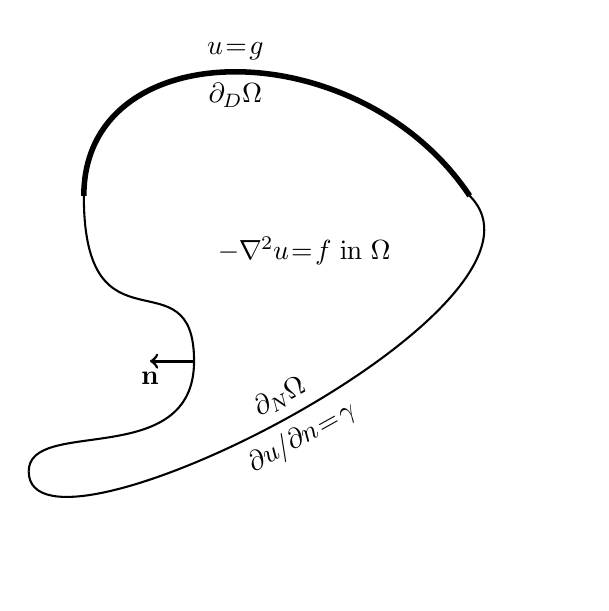
\begin{tikzpicture}[scale=0.7]
%\draw[gray,very thin] (-2,-6) grid (8,3);
\draw[line width=2pt] (0,0) .. controls (0,3) and (5,3) .. node[sloped,above] {$u=g$} node[sloped,below] {$\partial_D\Omega$} (7,0);
\draw[line width=0.75pt] (7,0) .. controls (9,-2) and (-1,-7) .. node[sloped,above] {$\partial_N\Omega$} node[sloped,below] {$\partial u/\partial n = \gamma$} (-1,-5);
\draw[line width=0.75pt] (-1,-5) .. controls (-1,-4) and (2,-5) .. (2,-3);
\draw[line width=0.75pt] (2,-3) .. controls (2,-1) and (0,-3) .. (0,0);
\draw[->,line width=1.0pt] (2,-3) -- (1.2,-3) node[below] {$\bn$}; % normal vector
\draw (4,-1) node {$- \grad^2 u = f$ in $\Omega$};
\end{tikzpicture}}
\begin{align}
- \grad^2 u &= f \quad \text{ on } \Omega, \label{poissonstrong} \\
u &= g \quad \text{ on } \partial_D \Omega, \notag \\
\frac{\partial u}{\partial n} &= \gamma \quad \text{ on } \partial_N \Omega \notag
\end{align}
where $\partial u/\partial n = \bn \cdot \grad u$ and $\bn$ is the outward unit normal on $\partial \Omega$.  The data of problem \eqref{poissonstrong}, besides the region $\Omega$ and its boundary, is a \emph{source term} $f\in L^2(\Omega)$, \emph{Dirichlet data} $g\in L^2(\partial_N \Omega)$, and \emph{non-homogeneous Neumann data} $\gamma\in L^2(\partial_N \Omega)$.

The Poisson problem models the distribution of temperature in a conducting object at steady state, the electrostatic potential, the equilibrium distribution from certain random walks, and many other other physical phenomena.  And it is linear, that is, if $u_1$ and $u_2$ are solutions then convex linear combinations are also solutions.  More relevantly, it is a linear problem in the sense that finite-dimensional approximations of the Poisson problem are simply matrix problems.

As \eqref{poissonstrong} is stated there may be no solution where ``$\grad^2 u$'' makes sense as a function, even for ``nice'' boundary and source functions.  In particular, there may be no $u\in C^2(\Omega)$ which is continuous up to the boundary (i.e.~$u\in C(\bar\Omega)$).  There is, however, a solution\sidenote{Many mathematical concepts, including a well-posedness proof that justifies this claim, are all covered by \citep{Evans}.  These are technicalities for us.  Our goal is computational performance in cases where the Poisson problem is mathematically well-behaved.} if we change to a \emph{weak formulation}.  Furthermore, if $\partial_D \Omega$ has positive measure then the solution is unique.  We will state the weak formulation after defining function spaces.

Define
    $$H^1(\Omega) = \{u\in L^2(\Omega) \big| \grad u \text{ exists a.e.~and } \grad u \in L^2(\Omega)\},$$
which is a Sobolev space \citep{Evans}.  This space has two subsets we will use, namely functions with value $g$ on $\partial_D \Omega$ and those with value $0$ on $\partial_D \Omega$, respectively, which we denote $H_g^1(\Omega)$ and $H_0^1(\Omega)$.  Note that $H_0^1(\Omega)$ is a linear subspace of $H^1(\Omega)$ while $H_g^1(\Omega)$ is generally not a subspace, because the zero function is not in it.  Nonetheless, from now on we refer to both $H_g^1(\Omega)$ and $H_0^1(\Omega)$ as ``subspaces''.

To get to the weak formulation of the Poisson problem we first choose any $v\in H_0^1(\Omega)$, multiply the first equation in \eqref{poissonstrong} by $v$, and integrate by parts:
\begin{equation*}
\int_\Omega \grad u \cdot \grad v - \int_{\partial\Omega} \frac{\partial u}{\partial n} v = \int_\Omega f v.
\end{equation*}
Now,\marginnote{%
{\color{red}Main ideas} of strong and weak formulations:\begin{itemize}
\item If $u \in H_g^1(\Omega)$ solves the strong form \eqref{poissonstrong} then it solves \eqref{poissonweak} also.
\item If $u \in H_g^1(\Omega)$ solves the weak form \eqref{poissonweak} then we accept it, by definition, as a solution of the Poisson problem.\end{itemize}} supposing we already have a classical solution $u$ of \eqref{poissonstrong}, which is in $H_g^1(\Omega)$, we use the other data, namely that $v=0$ on $\partial_D\Omega$ and that there is Neumann data $\gamma$ on $\partial_N\Omega$:
\begin{equation}
\int_\Omega \grad u \cdot \grad v = \int_\Omega f v + \int_{\partial_N\Omega} \gamma v\quad \text{ for any } v\in H_0^1(\Omega). \label{poissonweak}
\end{equation}

Equation \eqref{poissonweak} is the weak formulation of the Poisson problem.  A key observation is that $u$ itself incorporates the Dirichlet boundary condition, because it lives in $H_g^1(\Omega)$, while both the Neumann boundary data $\gamma$ and the source function $f$ appear in equation \eqref{poissonweak}.

The \emph{finite element method} (FEM) comes from requiring the weak formulation  \eqref{poissonweak} to be true for $u$ and $v$ in smaller, indeed finite-dimensional, subspaces of $H_g^1(\Omega)$ and $H_0^1(\Omega)$, respectively.  In our case these subspaces will be essentially the same, so our method is a \emph{Galerkin} FEM.  We will build these finite-dimensional subspaces, in the current example, using an unstructured triangulation on $\Omega\subset \RR^2$.  In particular, from now on in this chapter we restrict to $d=2$ dimensions.  Furthermore, to make our finite-dimensional spaces true subspaces of $H^1(\Omega)$---to make our FEM \emph{conforming}---we also require that $\Omega$ be polygonal, with $\partial\Omega$ a closed polygon.  We require that the segments in $\partial\Omega$ each have positive length, and be either entirely in $\partial_D\Omega$ or in $\partial_N\Omega$.

\begin{marginfigure}
\input{samplepoly.1.tikz}
\caption{A triangulation $\Th$ with $K=22$ triangles (elements) numbered $k=0,1,\dots,K-1$ ({\color{red} red}) and $N=16$ nodes numbered $j=0,1,\dots,N-1$  ({\color{blue} blue}).  Nodes $\bx_0$, $\bx_1$, $\bx_2$, $\bx_3$ are in the Dirichlet boundary $\partial_D\Omega$.}
\label{fig:number-elements}
\end{marginfigure}

By definition, a \emph{triangulation} is a set of non-overlapping, non-empty open triangles $\triangle_k\subset \RR^2$ which tile $\Omega$:
\begin{equation*}
\Th = \left\{\triangle_k \quad\Big|\quad \cup_k \overline{\triangle}_k = \overline{\Omega} \quad \text{ and} \quad \Omega_k \cap \Omega_l = \emptyset \text{ if } k\ne l\right\}.
\end{equation*}
There are $K$ triangles indexed $k=0,\dots,K-1$, as in Figure \ref{fig:number-elements}, for example.  (In contrast to \citet{Elmanetal2005}, which we generally follow but which implements in \Matlab, our indexing is always zero-based.  After all, we code in C.)  The subscript ``$h$'' in $\Th$ is traditional; it denotes the typical or maximum size $h$ (e.g.~diameter) of the triangles.  It serves as a reminder that we want to solve the Poisson problem accurately, that is, in the limit $h\to 0$.

We also index all the vertices (nodes) in the triangulation with $j=0,1,\dots,N$:
\begin{equation*}
\bx_j = (x_j,y_j).
\end{equation*}
An example of this node indexing is in Figure \ref{fig:number-elements}.

Later we will informally call the triangles \emph{elements}, though there is more to the definition of ``element,'' as we now explain.  We are going to approximate the Poisson problem with $\Pone$ finite elements, which means that our finite-dimensional subspace contains only piecewise-linear functions which are linear on each triangle $\triangle_k$.

In fact, for each node $j$ there is a $\Pone$ basis function, or ``hat'' function, $\phi_j(x,y)$ which is linear on each triangle, continuous on all of $\overline{\Omega}$, and equal to one on only one node $j$:\marginnote{%
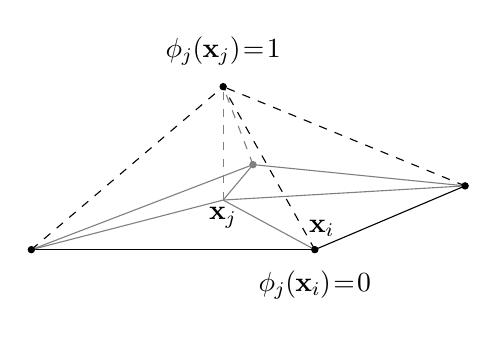
\begin{tikzpicture}[scale=0.9, z={(.707,.3)}]
    % (2,2,1) is top
    \draw[style=dashed] (0,0,0) -- (2,2,1); % to top from left
    \draw[style=dashed] (4,0,0) -- (2,2,1); %   ...  from front
    \draw[style=dashed] (4,0,3) -- (2,2,1); %   ...  from right
    \draw[color=gray, style=dashed] (0.3,0,4) -- (2,2,1); % from back
    \draw[color=gray, style=dashed] (2,0.4,1) -- (2,2,1); % from middle
    % draw base
    \draw (0,0,0) -- (4,0,0);
    \draw (4,0,0) -- (4,0,3);
    \draw[color=gray] (0,0,0) -- (0.3,0,4);
    \draw[color=gray] (0.3,0,4) -- (4,0,3);
    \draw[color=gray] (0,0,0) -- (2,0.4,1);
    \draw[color=gray] (2,0.4,1) -- (4,0,3);
    \draw[color=gray] (4,0,0) -- (2,0.4,1);
    \draw[color=gray] (2,0.4,1) -- (0.3,0,4);
    % draw \phi_j at nodes
    \filldraw (2,2,1) circle (1.25pt);
    \draw (2,2.5,1) node {$\phi_j(\bx_j)=1$};
    \draw (2,0.15,1) node {$\bx_j$};
    \filldraw (0,0,0) circle (1.25pt);
    \filldraw (4,0,0) circle (1.25pt);
    \draw (4,-0.5,0) node {$\phi_j(\bx_i)=0$};
    \draw (4.1,0.3,0) node {$\bx_i$};
    \filldraw (4,0,3) circle (1.25pt);
    \filldraw[color=gray] (0.3,0,4) circle (1.25pt);
\end{tikzpicture}
}%
\begin{equation*}
\phi_j(\bx_i) = \delta_{ij}.
\end{equation*}
The functions $\phi_j$ are in $H^1(\Omega)$, with piecewise-constant partial derivatives $\partial\phi_j/\partial x$ and $\partial\phi_j/\partial y$.  Also, the set $\{\phi_j\}_{j=0,\dots,N-1}$ is linearly-independent.  On each triangle, $\phi_j$ has three degrees of freedom:
\begin{equation*}
\phi_j(x,y) = A_k + B_k x + C_k y \quad \text{ on } \Delta_k.
\end{equation*}

We can immediately use these basis functions to approximate the Dirichlet data $g$ and ``extend'' it to the region $\Omega$.  We will assume from now on that the Dirichlet boundary is closed: $\partial_D\Omega = \overline{\partial_D\Omega}$.  Then we index the $L$ nodes which are in the Dirichlet boundary, $\bx_{j_l} \in \partial_D\Omega$ for $l=0,\dots,L-1$.  (Figure \ref{fig:number-elements} shows an example with $L=4$ and $j_l=l$ for $l=0,1,2,3$, but a general index $j_l$ is allowed.)  Then define an extended interpolant $\hat g$ of $g$ as the function which has the correct value on the Dirichlet boundary nodes and which extends to all of $\Omega$ in a continuous and piecewise-linear way:
\begin{equation}
\hat g(x,y) = \sum_{l=0,\dots,L} g(\bx_{j_l}) \phi_{j_l}(x,y). \label{hatgdefine}
\end{equation}

By using $\hat g$ and the basis functions $\phi_j$, we can now describe three finite-dimensional subspaces of $H^1(\Omega)$.  They are defined as the span of basis functions:\sidenote{Traditionally, basis functions for $S_g^h$, where $u_h$ lives, are called the \emph{trial} functions, and basis functions for $S_0^h$ are called \emph{test} functions.  We will generally just use the labels ``$S_g^h$'' and ``$S_0^h$.''}
\begin{align*}
S^h &= \Span\{\phi_j \,\big|\, \text{ all } j\,\}, \\
S_0^h &= \Span\{\phi_j \,\big|\, \bx_j \notin \partial_D \Omega\} \subset S^h, \\
S_g^h &= S_0^h + \hat g \subset S^h.
\end{align*}
Then $\dim(S^h)=N$ while $\dim(S_0^h)=\dim(S_g^h)=N-L$, with $S_g^h$ now clearly defined as an affine subspace of $S^h$.

Finally, our finite element method requires that the weak formulation  \eqref{poissonweak} be true of $u_h\in S_g^h$ for all $v\in S_0^h$.  Thus we first write $u_h$ in the above basis for $S_g^h$ using $N-L$ unknown coefficients $u_j$:
\begin{equation}
u_h(x,y) = \hat g(x,y) + \sum_{\bx_j \notin \partial_D \Omega} u_j\, \phi_j(x,y). \label{uhexpand}
\end{equation}
Then we require that the weak formulation hold for all $\phi_i$ in the above basis of $S_0^h$.  That is, using definition \eqref{hatgdefine} and expansion \eqref{uhexpand}, we require
\begin{align}
\sum_{j\big|\bx_j \notin \partial_D \Omega} u_j \int_\Omega \grad \phi_j \cdot \grad \phi_i &= \int_\Omega f \phi_i + \int_{\partial_N\Omega} \gamma \phi_i \label{poissonfem} \\
&\qquad - \sum_{l=0,\dots,L} g(\bx_{j_l})  \int_\Omega \grad \phi_{j_l} \cdot \grad \phi_i \notag
\end{align}
for all $i$ such that $\bx_i \notin \partial_D \Omega$.  The coefficients $u_j$, for all $j$ such that $\bx_j \notin \partial_D \Omega$, are unknown.

Note that the support (i.e.~nonzero set) of $\phi_j$ includes the node $\bx_j$ and all triangles (elements) $\triangle_k$ for which $\bx_j$ is a node of $\triangle_k$.  Thus the integral ``$\int_\Omega \grad \phi_j \cdot \grad \phi_i$'' in \eqref{poissonfem} is often zero.  Specifically, it is zero if nodes $\bx_i$ and $\bx_j$ are not connected by an edge in the triangulation, equivalently if $\bx_i$ and $\bx_j$ are not both nodes of at least one triangle in the triangulation.


\section{Assembling the matrix problem, element by element}

The finite-dimensional weak formulation \eqref{poissonfem} is simply a matrix equation.  For ease of construction we will include the node-wise Dirichlet conditions as rows of this matrix problem, so the matrix will have $N$ columns, corresponding to one unknown for \emph{every} node $\bx_j$, and $N$ rows.  We will then describe, and give a code for, \emph{assembling} this matrix equation.

Thus we define $A \in \RR^{N\times N}$ to have entries
\begin{equation*}
a_{ij} = \int_\Omega \grad \phi_j \cdot \grad \phi_i,
\end{equation*}
if $\bx_i \notin \partial_D \Omega$ and $\bx_j \notin \partial_D \Omega$.  Otherwise
\begin{equation*}
a_{ij} = \delta_{ij},
\end{equation*}
that is, in any row $i$ where $\bx_i \in \partial_D \Omega$ or column $j$ where $\bx_j \in \partial_D \Omega$.  (Notice that we index rows and columns of matrices and vectors starting with zero.)

We can immediately observe that $A$ is \emph{symmetric} because $a_{ij}=a_{ji}$.  Furthermore it is \emph{sparse}, that is, most entries are zero, as long as we consider triangulations with more than a handful of triangles.  These facts have profound consequences on the algorithms we will choose when solving a matrix equation
\begin{equation}
A \bu = \bb \label{poissonmatrix}
\end{equation}
using $A$.

Recalling \eqref{poissonfem}, the right side of our matrix equation ``$A \bu = \bb$'' will be a vector $\bb\in\RR^N$ with entries
    $$b_i = \int_\Omega f \phi_i + \int_{\partial_N\Omega} \gamma \phi_i - \sum_{l=0,\dots,L} g(\bx_{j_l})  \int_\Omega \grad \phi_{j_l} \cdot \grad \phi_i$$
if $\bx_i \notin \partial_D \Omega$ and
    $$b_i = g(\bx_{i})$$
if $\bx_i \in \partial_D \Omega$.

However, in practice we don't initially build $A$ quite as described in above.  We will initially build a matrix $\tilde A$ which ignors the type (i.e.~Dirichlet or Neumann) of the boundary nodes and computes all entries by the first formula above for $a_{ij}$.  That is, $\tilde A \in \RR^{N\times N}$ has entries
\begin{equation*}
\tilde a_{ij} = \int_\Omega \grad \phi_j \cdot \grad \phi_i
\end{equation*}
for all $i,j=0,1,\dots,N$.  Also we initially compute a right-hand side $\tilde \bb$ with simpler entries
    $$\tilde b_i = \int_\Omega f \phi_i + \int_{\partial_N\Omega} \gamma \phi_i$$
if $\bx_i \notin \partial_D \Omega$ and
    $$\tilde b_i = g(\bx_{i})$$
if $\bx_i \in \partial_D \Omega$.  Then we ``edit'' $\tilde A$ in each Dirichlet node \emph{row}, that is, for each $i$ where $\bx_i \in \partial_D \Omega$, simply by replacing the whole row by the corresponding row of the identity.  However, in each column $j$ for which $\bx_j \in \partial_D \Omega$, we move all entries $\tilde a_{ij}$ where $i$ is \emph{not} a Dirichlet row index, over to the right-hand side, multiplied by the negative of the boundary value $g(\bx_{j})$; informally we can write
    $$\tilde b_i \to \tilde b_i - g(\bx_{j}) \tilde a_{ij}$$
for the transformations which modify the initial version $\tilde \bb$.

After this ``editing'' stage is completed for all Dirichlet rows and columns, we get $A$ and $\bb$.  Since this part of the matrix assembly is a key stage of understanding our FEM codes, we give a concrete example to show the non-zero pattern of $A$.

\medskip\noindent\hrulefill
\begin{example} In Figure \ref{fig:squarefour} there are five nodes.  The $i=1,2$ nodes live in the (closed) Dirichlet boundary $\partial_D \Omega$.  The matrix $\tilde A$ has zero entries $\tilde a_{ij} = 0$ only where the integral $\int_\Omega \grad \phi_j \cdot \grad \phi_i=0$, which is somewhat rare in this small (coarse)-mesh case.  The nonzero values are simply marked ``$\X$'', and the zero entries are spaces:\begin{marginfigure}
\input{squarefour.tikz}
\caption{A triangulation of a square with five nodes.  The top segment is the Dirichlet boundary.}
\label{fig:squarefour}
\end{marginfigure}%
\begin{equation*}
\tilde A = \begin{bmatrix}
\X & \X &    & \X & \X \\
\X & \X & \X &    & \X \\
   & \X & \X & \X & \X \\
\X &    & \X & \X & \X \\
\X & \X & \X & \X & \X
\end{bmatrix}.
\end{equation*}
Now we color the $i=1,2$ or $j=1,2$ entries which will be edited:\marginnote{{\color{red} Potential gotcha}:  The first row of any matrix in this book is numbered ``$0$.''  Likewise the first column.}
\begin{equation*}
\tilde A = \begin{bmatrix}
\X & \redX &    & \X & \X \\
\blueX & \blueX & \blueX &    & \blueX \\
   & \blueX & \blueX & \blueX & \blueX \\
\X &    & \redX & \X & \X \\
\X & \redX & \redX & \X & \X
\end{bmatrix}.
\end{equation*}
The {\color{blue} blue} entries are changed to $0$ or $1$ so that these rows become rows of the identity; their computed values are tossed out.  The {\color{red} red} entries, specifically the four entries $\tilde a_{01}$, $\tilde a_{32}$, $\tilde a_{41}$, and $\tilde a_{42}$, are moved over to the right side, however, so their values are used.  In fact, we can give formulas for the $i=0,3,4$ entries of the final vector $\bb$ in terms of the initially-computed vector $\tilde\bb$,
\begin{align*}
b_0 &= \tilde b_0 - g(\bx_1) \tilde a_{01} \\
b_3 &= \tilde b_3 - g(\bx_2) \tilde a_{32} \\
b_4 &= \tilde b_4 - g(\bx_1) \tilde a_{41} - g(\bx_2) \tilde a_{42},
\end{align*}
while $b_1=\tilde b_1=g(\bx_1)$ and $b_2 = \tilde b_2 = g(\bx_2)$.  The final matrix $A$ has thereby been ``edited'' to be the identity matrix in rows $i=1,2$ and columns $j=1,2$; it has this pattern:
\begin{equation*}
A = \begin{bmatrix}
\X & & & \X & \X \\
 & \,1\, & & & \\
 & & \,1\, & & \\
\X & & & \X & \X \\
\X & & & \X & \X
\end{bmatrix}.
\end{equation*}
\end{example}
\noindent\hrulefill

\bigskip

In terms of later examples, it is useful to note that the initial construction is correct in the case where $\partial_D \Omega = \emptyset$ is empty.  Of course, in that case the Poisson problem does not have a unique solution because $u=(\text{constant})$ solves $-\grad^2 u=0$ with $\partial u/\partial n = 0$ on the whole boundary $\partial_N \Omega = \partial \Omega$.

\vspace{0.5in}
FIXME


\begin{align*}
\chi_0(\xi,\eta) &= 1-\xi-\eta \\
\chi_1(\xi,\eta) &= \xi \\
\chi_2(\xi,\eta) &= \eta
\end{align*}

$$\phi_i(x(\xi,\eta),y(\xi,\eta)) = \chi_i(\xi,\eta)$$

\begin{marginfigure}
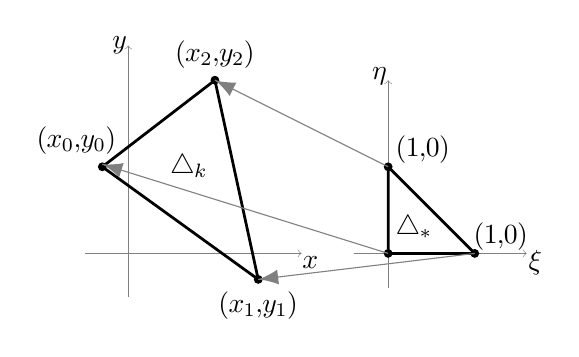
\begin{tikzpicture}[scale=1.1,
    decoration={
      markings,
      mark=at position 1 with {\arrow[scale=1.8,gray]{latex}};
    }]
% left x,y axes
    \draw[->, gray, very thin] (1.5,0) -- (4.0,0);
    \draw[->, gray, very thin] (2,-0.5) -- (2,2.4);
    \draw (4.1,-0.1) node {$x$};
    \draw (1.9,2.4) node {$y$};
    \filldraw (1.7,1) circle (1.25pt);    % (x_0,y_0)
    \filldraw (3.5,-0.3) circle (1.25pt); % (x_1,y_1)
    \filldraw (3.0,2.0) circle (1.25pt);  % (x_2,y_2)
    \draw (1.4,1.3) node {$(x_0,y_0)$};
    \draw (3.5,-0.6) node {$(x_1,y_1)$};
    \draw (3.0,2.3) node {$(x_2,y_2)$};
    \draw[line width=1pt] (1.7,1) -- (3.5,-0.3) -- (3.0,2.0) -- cycle;
    \draw (2.7,1.0) node {$\triangle_k$};
% right xi,eta axes
    \draw[->, gray, very thin] (4.6,0) -- (6.6,0);
    \draw[->, gray, very thin] (5,-0.4) -- (5,2.0);
    \draw (6.7,-0.1) node {$\xi$};
    \draw (4.9,2.05) node {$\eta$};
    \filldraw (5,0) circle (1.25pt);  % (0,0)
    \filldraw (6,0) circle (1.25pt);  % (1,0)
    \filldraw (5,1) circle (1.25pt);  % (0,1)
    \draw (6.3,0.2) node {$(1,0)$};
    \draw (5.4,1.2) node {$(1,0)$};
    \draw[line width=1pt] (5,0) -- (6,0) -- (5,1) -- cycle;
    \draw (5.3,0.3) node {$\triangle_\ast$};
% arcs connecting nodes
\draw[gray, postaction={decorate}] (5,0) -- (1.7,1.03);
\draw[gray, postaction={decorate}] (6,0) -- (3.5,-0.3);
\draw[gray, postaction={decorate}] (5,1) -- (3.0,2.0);
%\draw[thin, gray] (5,0) .. controls (4.7,0.4) and (2.0,1.1) .. (1.7,1);
\end{tikzpicture}
\medskip
\caption{Mapping of a $\Pone$ element $\triangle_k$ from the reference element $\triangle_\ast$.}
\label{fig:isoparametric}
\end{marginfigure}



\clearpage

\section{Getting a triangular mesh into \PETSc}

\begin{figure*}
% created by script tri2tikz.py command line:
%   ./tri2tikz.py --labelnodes --scale 2.0 --labeloffset 0.25 bump.1 bump.1.tikz
%
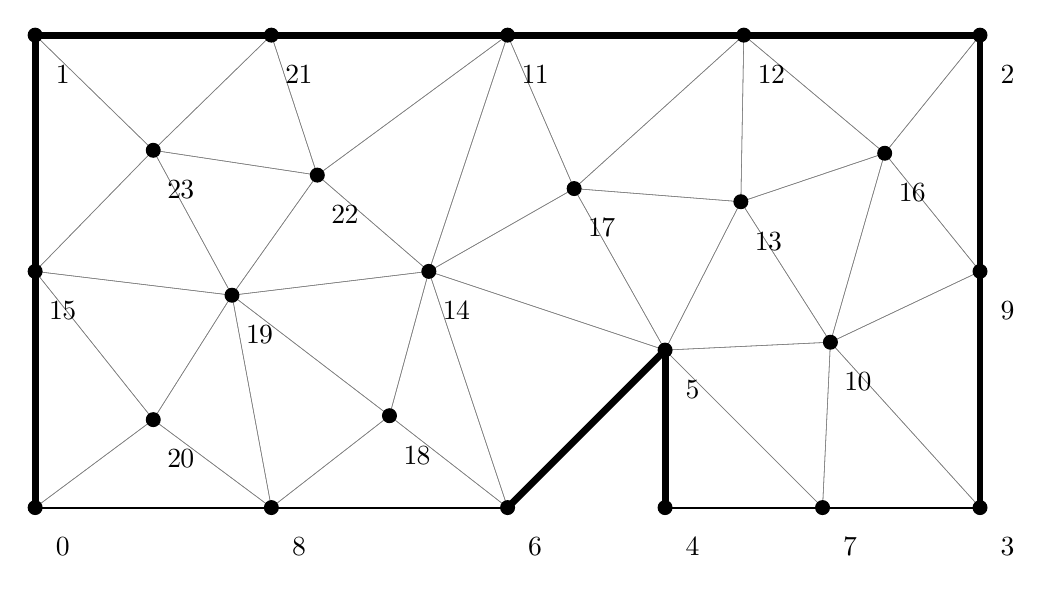
\begin{tikzpicture}[scale=2.000000]
  \draw[gray,very thin] (-1.500000,0.000000) -- (-2.250000,0.558372);
  \draw[gray,very thin] (-2.250000,0.558372) -- (-3.000000,0.000000);
  \draw[gray,very thin] (-3.000000,0.000000) -- (-1.500000,0.000000);
  \draw[gray,very thin] (-1.500000,0.000000) -- (0.000000,0.000000);
  \draw[gray,very thin] (0.000000,0.000000) -- (-0.750000,0.583333);
  \draw[gray,very thin] (-0.750000,0.583333) -- (-1.500000,0.000000);
  \draw[gray,very thin] (1.481325,1.942169) -- (0.422665,2.025778);
  \draw[gray,very thin] (0.422665,2.025778) -- (1.000000,1.000000);
  \draw[gray,very thin] (1.000000,1.000000) -- (1.481325,1.942169);
  \draw[gray,very thin] (-0.500000,1.500000) -- (0.000000,0.000000);
  \draw[gray,very thin] (0.000000,0.000000) -- (1.000000,1.000000);
  \draw[gray,very thin] (1.000000,1.000000) -- (-0.500000,1.500000);
  \draw[gray,very thin] (0.000000,3.000000) -- (-1.500000,3.000000);
  \draw[gray,very thin] (-1.500000,3.000000) -- (-1.208263,2.111158);
  \draw[gray,very thin] (-1.208263,2.111158) -- (0.000000,3.000000);
  \draw[gray,very thin] (2.000000,0.000000) -- (2.050000,1.050000);
  \draw[gray,very thin] (2.050000,1.050000) -- (1.000000,1.000000);
  \draw[gray,very thin] (1.000000,1.000000) -- (2.000000,0.000000);
  \draw[gray,very thin] (1.000000,0.000000) -- (2.000000,0.000000);
  \draw[gray,very thin] (2.000000,0.000000) -- (1.000000,1.000000);
  \draw[gray,very thin] (1.000000,1.000000) -- (1.000000,0.000000);
  \draw[gray,very thin] (2.394659,2.250000) -- (3.000000,1.500000);
  \draw[gray,very thin] (3.000000,1.500000) -- (3.000000,3.000000);
  \draw[gray,very thin] (3.000000,3.000000) -- (2.394659,2.250000);
  \draw[gray,very thin] (1.500000,3.000000) -- (0.422665,2.025778);
  \draw[gray,very thin] (0.422665,2.025778) -- (1.481325,1.942169);
  \draw[gray,very thin] (1.481325,1.942169) -- (1.500000,3.000000);
  \draw[gray,very thin] (2.050000,1.050000) -- (3.000000,0.000000);
  \draw[gray,very thin] (3.000000,0.000000) -- (3.000000,1.500000);
  \draw[gray,very thin] (3.000000,1.500000) -- (2.050000,1.050000);
  \draw[gray,very thin] (2.394659,2.250000) -- (2.050000,1.050000);
  \draw[gray,very thin] (2.050000,1.050000) -- (3.000000,1.500000);
  \draw[gray,very thin] (3.000000,1.500000) -- (2.394659,2.250000);
  \draw[gray,very thin] (-1.500000,3.000000) -- (-3.000000,3.000000);
  \draw[gray,very thin] (-3.000000,3.000000) -- (-2.250000,2.268853);
  \draw[gray,very thin] (-2.250000,2.268853) -- (-1.500000,3.000000);
  \draw[gray,very thin] (1.481325,1.942169) -- (1.000000,1.000000);
  \draw[gray,very thin] (1.000000,1.000000) -- (2.050000,1.050000);
  \draw[gray,very thin] (2.050000,1.050000) -- (1.481325,1.942169);
  \draw[gray,very thin] (3.000000,0.000000) -- (2.050000,1.050000);
  \draw[gray,very thin] (2.050000,1.050000) -- (2.000000,0.000000);
  \draw[gray,very thin] (2.000000,0.000000) -- (3.000000,0.000000);
  \draw[gray,very thin] (0.422665,2.025778) -- (1.500000,3.000000);
  \draw[gray,very thin] (1.500000,3.000000) -- (0.000000,3.000000);
  \draw[gray,very thin] (0.000000,3.000000) -- (0.422665,2.025778);
  \draw[gray,very thin] (2.394659,2.250000) -- (1.500000,3.000000);
  \draw[gray,very thin] (1.500000,3.000000) -- (1.481325,1.942169);
  \draw[gray,very thin] (1.481325,1.942169) -- (2.394659,2.250000);
  \draw[gray,very thin] (-1.750000,1.348485) -- (-0.750000,0.583333);
  \draw[gray,very thin] (-0.750000,0.583333) -- (-0.500000,1.500000);
  \draw[gray,very thin] (-0.500000,1.500000) -- (-1.750000,1.348485);
  \draw[gray,very thin] (-1.500000,0.000000) -- (-0.750000,0.583333);
  \draw[gray,very thin] (-0.750000,0.583333) -- (-1.750000,1.348485);
  \draw[gray,very thin] (-1.750000,1.348485) -- (-1.500000,0.000000);
  \draw[gray,very thin] (1.500000,3.000000) -- (2.394659,2.250000);
  \draw[gray,very thin] (2.394659,2.250000) -- (3.000000,3.000000);
  \draw[gray,very thin] (3.000000,3.000000) -- (1.500000,3.000000);
  \draw[gray,very thin] (2.050000,1.050000) -- (2.394659,2.250000);
  \draw[gray,very thin] (2.394659,2.250000) -- (1.481325,1.942169);
  \draw[gray,very thin] (1.481325,1.942169) -- (2.050000,1.050000);
  \draw[gray,very thin] (0.000000,3.000000) -- (-0.500000,1.500000);
  \draw[gray,very thin] (-0.500000,1.500000) -- (0.422665,2.025778);
  \draw[gray,very thin] (0.422665,2.025778) -- (0.000000,3.000000);
  \draw[gray,very thin] (1.000000,1.000000) -- (0.422665,2.025778);
  \draw[gray,very thin] (0.422665,2.025778) -- (-0.500000,1.500000);
  \draw[gray,very thin] (-0.500000,1.500000) -- (1.000000,1.000000);
  \draw[gray,very thin] (0.000000,0.000000) -- (-0.500000,1.500000);
  \draw[gray,very thin] (-0.500000,1.500000) -- (-0.750000,0.583333);
  \draw[gray,very thin] (-0.750000,0.583333) -- (0.000000,0.000000);
  \draw[gray,very thin] (-1.750000,1.348485) -- (-2.250000,2.268853);
  \draw[gray,very thin] (-2.250000,2.268853) -- (-3.000000,1.500000);
  \draw[gray,very thin] (-3.000000,1.500000) -- (-1.750000,1.348485);
  \draw[gray,very thin] (-3.000000,1.500000) -- (-3.000000,0.000000);
  \draw[gray,very thin] (-3.000000,0.000000) -- (-2.250000,0.558372);
  \draw[gray,very thin] (-2.250000,0.558372) -- (-3.000000,1.500000);
  \draw[gray,very thin] (-1.500000,0.000000) -- (-1.750000,1.348485);
  \draw[gray,very thin] (-1.750000,1.348485) -- (-2.250000,0.558372);
  \draw[gray,very thin] (-2.250000,0.558372) -- (-1.500000,0.000000);
  \draw[gray,very thin] (-3.000000,1.500000) -- (-2.250000,0.558372);
  \draw[gray,very thin] (-2.250000,0.558372) -- (-1.750000,1.348485);
  \draw[gray,very thin] (-1.750000,1.348485) -- (-3.000000,1.500000);
  \draw[gray,very thin] (0.000000,3.000000) -- (-1.208263,2.111158);
  \draw[gray,very thin] (-1.208263,2.111158) -- (-0.500000,1.500000);
  \draw[gray,very thin] (-0.500000,1.500000) -- (0.000000,3.000000);
  \draw[gray,very thin] (-0.500000,1.500000) -- (-1.208263,2.111158);
  \draw[gray,very thin] (-1.208263,2.111158) -- (-1.750000,1.348485);
  \draw[gray,very thin] (-1.750000,1.348485) -- (-0.500000,1.500000);
  \draw[gray,very thin] (-2.250000,2.268853) -- (-1.208263,2.111158);
  \draw[gray,very thin] (-1.208263,2.111158) -- (-1.500000,3.000000);
  \draw[gray,very thin] (-1.500000,3.000000) -- (-2.250000,2.268853);
  \draw[gray,very thin] (-3.000000,1.500000) -- (-2.250000,2.268853);
  \draw[gray,very thin] (-2.250000,2.268853) -- (-3.000000,3.000000);
  \draw[gray,very thin] (-3.000000,3.000000) -- (-3.000000,1.500000);
  \draw[gray,very thin] (-1.208263,2.111158) -- (-2.250000,2.268853);
  \draw[gray,very thin] (-2.250000,2.268853) -- (-1.750000,1.348485);
  \draw[gray,very thin] (-1.750000,1.348485) -- (-1.208263,2.111158);
  \draw[line width=2.5pt] (-3.000000,0.000000) -- (-3.000000,1.500000);
  \draw[line width=2.5pt] (-3.000000,3.000000) -- (-1.500000,3.000000);
  \draw[line width=2.5pt] (3.000000,3.000000) -- (3.000000,1.500000);
  \draw[line width=0.75pt] (3.000000,0.000000) -- (2.000000,0.000000);
  \draw[line width=0.75pt] (2.000000,0.000000) -- (1.000000,0.000000);
  \draw[line width=2.5pt] (1.000000,1.000000) -- (1.000000,0.000000);
  \draw[line width=2.5pt] (0.000000,0.000000) -- (1.000000,1.000000);
  \draw[line width=0.75pt] (0.000000,0.000000) -- (-1.500000,0.000000);
  \draw[line width=0.75pt] (-1.500000,0.000000) -- (-3.000000,0.000000);
  \draw[line width=2.5pt] (3.000000,1.500000) -- (3.000000,0.000000);
  \draw[line width=2.5pt] (0.000000,3.000000) -- (1.500000,3.000000);
  \draw[line width=2.5pt] (1.500000,3.000000) -- (3.000000,3.000000);
  \draw[line width=2.5pt] (-3.000000,1.500000) -- (-3.000000,3.000000);
  \draw[line width=2.5pt] (-1.500000,3.000000) -- (0.000000,3.000000);
  \draw (-2.825000,-0.250000) node {$0$};
  \filldraw (-3.000000,0.000000) circle (1.25pt);
  \draw (-2.825000,2.750000) node {$1$};
  \filldraw (-3.000000,3.000000) circle (1.25pt);
  \draw (3.175000,2.750000) node {$2$};
  \filldraw (3.000000,3.000000) circle (1.25pt);
  \draw (3.175000,-0.250000) node {$3$};
  \filldraw (3.000000,0.000000) circle (1.25pt);
  \draw (1.175000,-0.250000) node {$4$};
  \filldraw (1.000000,0.000000) circle (1.25pt);
  \draw (1.175000,0.750000) node {$5$};
  \filldraw (1.000000,1.000000) circle (1.25pt);
  \draw (0.175000,-0.250000) node {$6$};
  \filldraw (0.000000,0.000000) circle (1.25pt);
  \draw (2.175000,-0.250000) node {$7$};
  \filldraw (2.000000,0.000000) circle (1.25pt);
  \draw (-1.325000,-0.250000) node {$8$};
  \filldraw (-1.500000,0.000000) circle (1.25pt);
  \draw (3.175000,1.250000) node {$9$};
  \filldraw (3.000000,1.500000) circle (1.25pt);
  \draw (2.225000,0.800000) node {$10$};
  \filldraw (2.050000,1.050000) circle (1.25pt);
  \draw (0.175000,2.750000) node {$11$};
  \filldraw (0.000000,3.000000) circle (1.25pt);
  \draw (1.675000,2.750000) node {$12$};
  \filldraw (1.500000,3.000000) circle (1.25pt);
  \draw (1.656325,1.692169) node {$13$};
  \filldraw (1.481325,1.942169) circle (1.25pt);
  \draw (-0.325000,1.250000) node {$14$};
  \filldraw (-0.500000,1.500000) circle (1.25pt);
  \draw (-2.825000,1.250000) node {$15$};
  \filldraw (-3.000000,1.500000) circle (1.25pt);
  \draw (2.569659,2.000000) node {$16$};
  \filldraw (2.394659,2.250000) circle (1.25pt);
  \draw (0.597665,1.775778) node {$17$};
  \filldraw (0.422665,2.025778) circle (1.25pt);
  \draw (-0.575000,0.333333) node {$18$};
  \filldraw (-0.750000,0.583333) circle (1.25pt);
  \draw (-1.575000,1.098485) node {$19$};
  \filldraw (-1.750000,1.348485) circle (1.25pt);
  \draw (-2.075000,0.308372) node {$20$};
  \filldraw (-2.250000,0.558372) circle (1.25pt);
  \draw (-1.325000,2.750000) node {$21$};
  \filldraw (-1.500000,3.000000) circle (1.25pt);
  \draw (-1.033263,1.861158) node {$22$};
  \filldraw (-1.208263,2.111158) circle (1.25pt);
  \draw (-2.075000,2.018853) node {$23$};
  \filldraw (-2.250000,2.268853) circle (1.25pt);
\end{tikzpicture}

\caption{A FEM triangulation.  Nodes are labeled by $j=0,\dots,N-1$ with $N=24$.  The Dirichlet boundary $\partial_D \Omega$ is bold.}
\label{fig:triangulation}
\end{figure*}

\begin{figure*}
% created by script tri2tikz.py command line:
%   ./tri2tikz.py --scale 2.0 bump.2 bump.2.tikz
%
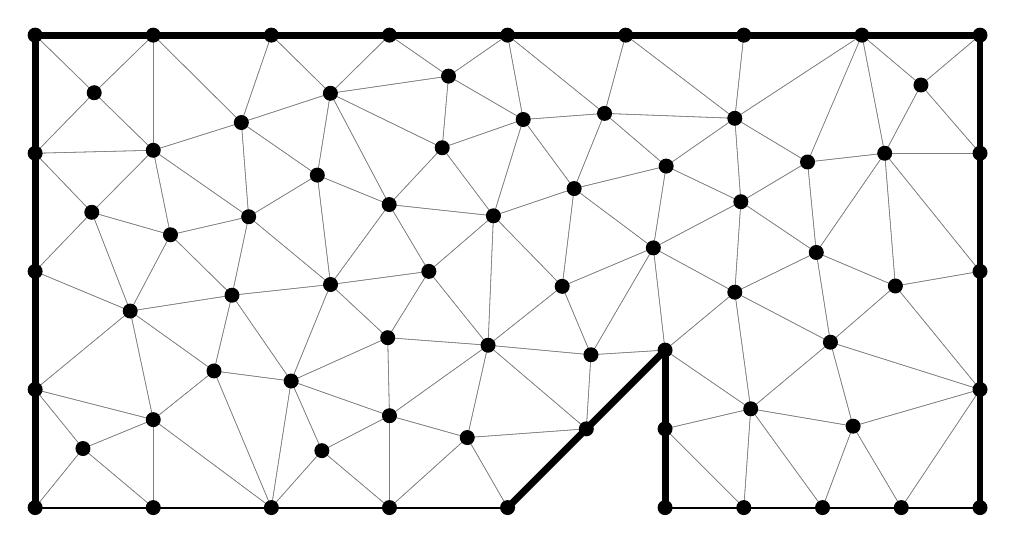
\begin{tikzpicture}[scale=2.000000]
  \draw[gray,very thin] (-1.500000,0.000000) -- (-2.250000,0.558372);
  \draw[gray,very thin] (-2.250000,0.558372) -- (-2.250000,0.000000);
  \draw[gray,very thin] (-2.250000,0.000000) -- (-1.500000,0.000000);
  \draw[gray,very thin] (0.000000,0.000000) -- (-0.256051,0.444601);
  \draw[gray,very thin] (-0.256051,0.444601) -- (-0.750000,0.000000);
  \draw[gray,very thin] (-0.750000,0.000000) -- (0.000000,0.000000);
  \draw[gray,very thin] (0.346751,1.404919) -- (0.925557,1.649218);
  \draw[gray,very thin] (0.925557,1.649218) -- (0.422665,2.025778);
  \draw[gray,very thin] (0.422665,2.025778) -- (0.346751,1.404919);
  \draw[gray,very thin] (-0.761257,1.078828) -- (-0.750000,0.583333);
  \draw[gray,very thin] (-0.750000,0.583333) -- (-0.123947,1.031029);
  \draw[gray,very thin] (-0.123947,1.031029) -- (-0.761257,1.078828);
  \draw[gray,very thin] (-0.750000,3.000000) -- (-1.500000,3.000000);
  \draw[gray,very thin] (-1.500000,3.000000) -- (-1.125000,2.630785);
  \draw[gray,very thin] (-1.125000,2.630785) -- (-0.750000,3.000000);
  \draw[gray,very thin] (1.543942,0.627219) -- (2.194079,0.516949);
  \draw[gray,very thin] (2.194079,0.516949) -- (2.050000,1.050000);
  \draw[gray,very thin] (2.050000,1.050000) -- (1.543942,0.627219);
  \draw[gray,very thin] (2.194079,0.516949) -- (1.543942,0.627219);
  \draw[gray,very thin] (1.543942,0.627219) -- (2.000000,0.000000);
  \draw[gray,very thin] (2.000000,0.000000) -- (2.194079,0.516949);
  \draw[gray,very thin] (3.000000,3.000000) -- (2.625000,2.683379);
  \draw[gray,very thin] (2.625000,2.683379) -- (3.000000,2.250000);
  \draw[gray,very thin] (3.000000,2.250000) -- (3.000000,3.000000);
  \draw[gray,very thin] (0.750000,3.000000) -- (1.442878,2.471928);
  \draw[gray,very thin] (1.442878,2.471928) -- (1.500000,3.000000);
  \draw[gray,very thin] (1.500000,3.000000) -- (0.750000,3.000000);
  \draw[gray,very thin] (3.000000,0.750000) -- (2.462433,1.407086);
  \draw[gray,very thin] (2.462433,1.407086) -- (2.050000,1.050000);
  \draw[gray,very thin] (2.050000,1.050000) -- (3.000000,0.750000);
  \draw[gray,very thin] (2.462433,1.407086) -- (2.394659,2.250000);
  \draw[gray,very thin] (2.394659,2.250000) -- (1.960192,1.620079);
  \draw[gray,very thin] (1.960192,1.620079) -- (2.462433,1.407086);
  \draw[gray,very thin] (-2.625000,2.634426) -- (-2.250000,2.268853);
  \draw[gray,very thin] (-2.250000,2.268853) -- (-2.250000,3.000000);
  \draw[gray,very thin] (-2.250000,3.000000) -- (-2.625000,2.634426);
  \draw[gray,very thin] (2.050000,1.050000) -- (1.960192,1.620079);
  \draw[gray,very thin] (1.960192,1.620079) -- (1.442775,1.367831);
  \draw[gray,very thin] (1.442775,1.367831) -- (2.050000,1.050000);
  \draw[gray,very thin] (3.000000,0.750000) -- (2.500000,0.000000);
  \draw[gray,very thin] (2.500000,0.000000) -- (3.000000,0.000000);
  \draw[gray,very thin] (3.000000,0.000000) -- (3.000000,0.750000);
  \draw[gray,very thin] (0.099254,2.464264) -- (0.422665,2.025778);
  \draw[gray,very thin] (0.422665,2.025778) -- (0.615679,2.503029);
  \draw[gray,very thin] (0.615679,2.503029) -- (0.099254,2.464264);
  \draw[gray,very thin] (1.904813,2.194525) -- (1.442878,2.471928);
  \draw[gray,very thin] (1.442878,2.471928) -- (1.481325,1.942169);
  \draw[gray,very thin] (1.481325,1.942169) -- (1.904813,2.194525);
  \draw[gray,very thin] (-1.124060,1.416490) -- (-0.500000,1.500000);
  \draw[gray,very thin] (-0.500000,1.500000) -- (-0.751743,1.924235);
  \draw[gray,very thin] (-0.751743,1.924235) -- (-1.124060,1.416490);
  \draw[gray,very thin] (-0.761257,1.078828) -- (-1.374144,0.803661);
  \draw[gray,very thin] (-1.374144,0.803661) -- (-0.750000,0.583333);
  \draw[gray,very thin] (-0.750000,0.583333) -- (-0.761257,1.078828);
  \draw[gray,very thin] (2.250000,3.000000) -- (1.442878,2.471928);
  \draw[gray,very thin] (1.442878,2.471928) -- (1.904813,2.194525);
  \draw[gray,very thin] (1.904813,2.194525) -- (2.250000,3.000000);
  \draw[gray,very thin] (1.904813,2.194525) -- (1.960192,1.620079);
  \draw[gray,very thin] (1.960192,1.620079) -- (2.394659,2.250000);
  \draw[gray,very thin] (2.394659,2.250000) -- (1.904813,2.194525);
  \draw[gray,very thin] (-0.089889,1.852775) -- (0.099254,2.464264);
  \draw[gray,very thin] (0.099254,2.464264) -- (-0.415249,2.284959);
  \draw[gray,very thin] (-0.415249,2.284959) -- (-0.089889,1.852775);
  \draw[gray,very thin] (-0.089889,1.852775) -- (-0.500000,1.500000);
  \draw[gray,very thin] (-0.500000,1.500000) -- (-0.123947,1.031029);
  \draw[gray,very thin] (-0.123947,1.031029) -- (-0.089889,1.852775);
  \draw[gray,very thin] (-0.123947,1.031029) -- (-0.750000,0.583333);
  \draw[gray,very thin] (-0.750000,0.583333) -- (-0.256051,0.444601);
  \draw[gray,very thin] (-0.256051,0.444601) -- (-0.123947,1.031029);
  \draw[gray,very thin] (-2.396353,1.248078) -- (-2.140597,1.732288);
  \draw[gray,very thin] (-2.140597,1.732288) -- (-2.640264,1.875000);
  \draw[gray,very thin] (-2.640264,1.875000) -- (-2.396353,1.248078);
  \draw[gray,very thin] (-3.000000,0.750000) -- (-3.000000,0.000000);
  \draw[gray,very thin] (-3.000000,0.000000) -- (-2.696333,0.375000);
  \draw[gray,very thin] (-2.696333,0.375000) -- (-3.000000,0.750000);
  \draw[gray,very thin] (-1.864316,0.867565) -- (-1.500000,0.000000);
  \draw[gray,very thin] (-1.500000,0.000000) -- (-1.374144,0.803661);
  \draw[gray,very thin] (-1.374144,0.803661) -- (-1.864316,0.867565);
  \draw[gray,very thin] (-1.864316,0.867565) -- (-2.396353,1.248078);
  \draw[gray,very thin] (-2.396353,1.248078) -- (-2.250000,0.558372);
  \draw[gray,very thin] (-2.250000,0.558372) -- (-1.864316,0.867565);
  \draw[gray,very thin] (-0.415249,2.284959) -- (-0.375000,2.739680);
  \draw[gray,very thin] (-0.375000,2.739680) -- (-1.125000,2.630785);
  \draw[gray,very thin] (-1.125000,2.630785) -- (-0.415249,2.284959);
  \draw[gray,very thin] (-1.124060,1.416490) -- (-0.751743,1.924235);
  \draw[gray,very thin] (-0.751743,1.924235) -- (-1.208263,2.111158);
  \draw[gray,very thin] (-1.208263,2.111158) -- (-1.124060,1.416490);
  \draw[gray,very thin] (-1.690505,2.445174) -- (-1.500000,3.000000);
  \draw[gray,very thin] (-1.500000,3.000000) -- (-2.250000,3.000000);
  \draw[gray,very thin] (-2.250000,3.000000) -- (-1.690505,2.445174);
  \draw[gray,very thin] (-2.250000,2.268853) -- (-2.625000,2.634426);
  \draw[gray,very thin] (-2.625000,2.634426) -- (-3.000000,2.250000);
  \draw[gray,very thin] (-3.000000,2.250000) -- (-2.250000,2.268853);
  \draw[gray,very thin] (-2.140597,1.732288) -- (-1.644051,1.846966);
  \draw[gray,very thin] (-1.644051,1.846966) -- (-2.250000,2.268853);
  \draw[gray,very thin] (-2.250000,2.268853) -- (-2.140597,1.732288);
  \draw[gray,very thin] (-2.696333,0.375000) -- (-2.250000,0.000000);
  \draw[gray,very thin] (-2.250000,0.000000) -- (-2.250000,0.558372);
  \draw[gray,very thin] (-2.250000,0.558372) -- (-2.696333,0.375000);
  \draw[gray,very thin] (-1.179284,0.361460) -- (-0.750000,0.000000);
  \draw[gray,very thin] (-0.750000,0.000000) -- (-0.750000,0.583333);
  \draw[gray,very thin] (-0.750000,0.583333) -- (-1.179284,0.361460);
  \draw[gray,very thin] (-1.690505,2.445174) -- (-1.125000,2.630785);
  \draw[gray,very thin] (-1.125000,2.630785) -- (-1.500000,3.000000);
  \draw[gray,very thin] (-1.500000,3.000000) -- (-1.690505,2.445174);
  \draw[gray,very thin] (-0.751743,1.924235) -- (-1.125000,2.630785);
  \draw[gray,very thin] (-1.125000,2.630785) -- (-1.208263,2.111158);
  \draw[gray,very thin] (-1.208263,2.111158) -- (-0.751743,1.924235);
  \draw[gray,very thin] (-1.125000,2.630785) -- (-0.751743,1.924235);
  \draw[gray,very thin] (-0.751743,1.924235) -- (-0.415249,2.284959);
  \draw[gray,very thin] (-0.415249,2.284959) -- (-1.125000,2.630785);
  \draw[gray,very thin] (-0.415249,2.284959) -- (-0.751743,1.924235);
  \draw[gray,very thin] (-0.751743,1.924235) -- (-0.089889,1.852775);
  \draw[gray,very thin] (-0.089889,1.852775) -- (-0.415249,2.284959);
  \draw[gray,very thin] (0.000000,3.000000) -- (-0.750000,3.000000);
  \draw[gray,very thin] (-0.750000,3.000000) -- (-0.375000,2.739680);
  \draw[gray,very thin] (-0.375000,2.739680) -- (0.000000,3.000000);
  \draw[gray,very thin] (-1.208263,2.111158) -- (-1.644051,1.846966);
  \draw[gray,very thin] (-1.644051,1.846966) -- (-1.124060,1.416490);
  \draw[gray,very thin] (-1.124060,1.416490) -- (-1.208263,2.111158);
  \draw[gray,very thin] (-0.089889,1.852775) -- (-0.751743,1.924235);
  \draw[gray,very thin] (-0.751743,1.924235) -- (-0.500000,1.500000);
  \draw[gray,very thin] (-0.500000,1.500000) -- (-0.089889,1.852775);
  \draw[gray,very thin] (-1.374144,0.803661) -- (-1.124060,1.416490);
  \draw[gray,very thin] (-1.124060,1.416490) -- (-1.750000,1.348485);
  \draw[gray,very thin] (-1.750000,1.348485) -- (-1.374144,0.803661);
  \draw[gray,very thin] (-0.761257,1.078828) -- (-1.124060,1.416490);
  \draw[gray,very thin] (-1.124060,1.416490) -- (-1.374144,0.803661);
  \draw[gray,very thin] (-1.374144,0.803661) -- (-0.761257,1.078828);
  \draw[gray,very thin] (-1.864316,0.867565) -- (-1.374144,0.803661);
  \draw[gray,very thin] (-1.374144,0.803661) -- (-1.750000,1.348485);
  \draw[gray,very thin] (-1.750000,1.348485) -- (-1.864316,0.867565);
  \draw[gray,very thin] (-1.500000,0.000000) -- (-1.179284,0.361460);
  \draw[gray,very thin] (-1.179284,0.361460) -- (-1.374144,0.803661);
  \draw[gray,very thin] (-1.374144,0.803661) -- (-1.500000,0.000000);
  \draw[gray,very thin] (-0.256051,0.444601) -- (0.000000,0.000000);
  \draw[gray,very thin] (0.000000,0.000000) -- (0.500000,0.500000);
  \draw[gray,very thin] (0.500000,0.500000) -- (-0.256051,0.444601);
  \draw[gray,very thin] (-0.500000,1.500000) -- (-1.124060,1.416490);
  \draw[gray,very thin] (-1.124060,1.416490) -- (-0.761257,1.078828);
  \draw[gray,very thin] (-0.761257,1.078828) -- (-0.500000,1.500000);
  \draw[gray,very thin] (1.000000,1.000000) -- (0.529558,0.970442);
  \draw[gray,very thin] (0.529558,0.970442) -- (0.500000,0.500000);
  \draw[gray,very thin] (0.500000,0.500000) -- (1.000000,1.000000);
  \draw[gray,very thin] (-0.089889,1.852775) -- (0.346751,1.404919);
  \draw[gray,very thin] (0.346751,1.404919) -- (0.422665,2.025778);
  \draw[gray,very thin] (0.422665,2.025778) -- (-0.089889,1.852775);
  \draw[gray,very thin] (-2.396353,1.248078) -- (-1.864316,0.867565);
  \draw[gray,very thin] (-1.864316,0.867565) -- (-1.750000,1.348485);
  \draw[gray,very thin] (-1.750000,1.348485) -- (-2.396353,1.248078);
  \draw[gray,very thin] (-1.500000,0.000000) -- (-1.864316,0.867565);
  \draw[gray,very thin] (-1.864316,0.867565) -- (-2.250000,0.558372);
  \draw[gray,very thin] (-2.250000,0.558372) -- (-1.500000,0.000000);
  \draw[gray,very thin] (-2.140597,1.732288) -- (-2.396353,1.248078);
  \draw[gray,very thin] (-2.396353,1.248078) -- (-1.750000,1.348485);
  \draw[gray,very thin] (-1.750000,1.348485) -- (-2.140597,1.732288);
  \draw[gray,very thin] (-2.396353,1.248078) -- (-3.000000,1.500000);
  \draw[gray,very thin] (-3.000000,1.500000) -- (-3.000000,0.750000);
  \draw[gray,very thin] (-3.000000,0.750000) -- (-2.396353,1.248078);
  \draw[gray,very thin] (-0.750000,0.000000) -- (-1.179284,0.361460);
  \draw[gray,very thin] (-1.179284,0.361460) -- (-1.500000,0.000000);
  \draw[gray,very thin] (-1.500000,0.000000) -- (-0.750000,0.000000);
  \draw[gray,very thin] (-0.750000,0.583333) -- (-1.374144,0.803661);
  \draw[gray,very thin] (-1.374144,0.803661) -- (-1.179284,0.361460);
  \draw[gray,very thin] (-1.179284,0.361460) -- (-0.750000,0.583333);
  \draw[gray,very thin] (-1.644051,1.846966) -- (-2.140597,1.732288);
  \draw[gray,very thin] (-2.140597,1.732288) -- (-1.750000,1.348485);
  \draw[gray,very thin] (-1.750000,1.348485) -- (-1.644051,1.846966);
  \draw[gray,very thin] (-2.250000,2.268853) -- (-3.000000,2.250000);
  \draw[gray,very thin] (-3.000000,2.250000) -- (-2.640264,1.875000);
  \draw[gray,very thin] (-2.640264,1.875000) -- (-2.250000,2.268853);
  \draw[gray,very thin] (-1.124060,1.416490) -- (-1.644051,1.846966);
  \draw[gray,very thin] (-1.644051,1.846966) -- (-1.750000,1.348485);
  \draw[gray,very thin] (-1.750000,1.348485) -- (-1.124060,1.416490);
  \draw[gray,very thin] (-1.644051,1.846966) -- (-1.208263,2.111158);
  \draw[gray,very thin] (-1.208263,2.111158) -- (-1.690505,2.445174);
  \draw[gray,very thin] (-1.690505,2.445174) -- (-1.644051,1.846966);
  \draw[gray,very thin] (-0.761257,1.078828) -- (-0.123947,1.031029);
  \draw[gray,very thin] (-0.123947,1.031029) -- (-0.500000,1.500000);
  \draw[gray,very thin] (-0.500000,1.500000) -- (-0.761257,1.078828);
  \draw[gray,very thin] (0.099254,2.464264) -- (-0.089889,1.852775);
  \draw[gray,very thin] (-0.089889,1.852775) -- (0.422665,2.025778);
  \draw[gray,very thin] (0.422665,2.025778) -- (0.099254,2.464264);
  \draw[gray,very thin] (0.500000,0.500000) -- (0.529558,0.970442);
  \draw[gray,very thin] (0.529558,0.970442) -- (-0.123947,1.031029);
  \draw[gray,very thin] (-0.123947,1.031029) -- (0.500000,0.500000);
  \draw[gray,very thin] (0.925557,1.649218) -- (1.481325,1.942169);
  \draw[gray,very thin] (1.481325,1.942169) -- (1.006948,2.168468);
  \draw[gray,very thin] (1.006948,2.168468) -- (0.925557,1.649218);
  \draw[gray,very thin] (0.529558,0.970442) -- (0.925557,1.649218);
  \draw[gray,very thin] (0.925557,1.649218) -- (0.346751,1.404919);
  \draw[gray,very thin] (0.346751,1.404919) -- (0.529558,0.970442);
  \draw[gray,very thin] (1.442775,1.367831) -- (0.925557,1.649218);
  \draw[gray,very thin] (0.925557,1.649218) -- (1.000000,1.000000);
  \draw[gray,very thin] (1.000000,1.000000) -- (1.442775,1.367831);
  \draw[gray,very thin] (0.422665,2.025778) -- (1.006948,2.168468);
  \draw[gray,very thin] (1.006948,2.168468) -- (0.615679,2.503029);
  \draw[gray,very thin] (0.615679,2.503029) -- (0.422665,2.025778);
  \draw[gray,very thin] (-0.375000,2.739680) -- (0.099254,2.464264);
  \draw[gray,very thin] (0.099254,2.464264) -- (0.000000,3.000000);
  \draw[gray,very thin] (0.000000,3.000000) -- (-0.375000,2.739680);
  \draw[gray,very thin] (0.422665,2.025778) -- (0.925557,1.649218);
  \draw[gray,very thin] (0.925557,1.649218) -- (1.006948,2.168468);
  \draw[gray,very thin] (1.006948,2.168468) -- (0.422665,2.025778);
  \draw[gray,very thin] (0.615679,2.503029) -- (0.000000,3.000000);
  \draw[gray,very thin] (0.000000,3.000000) -- (0.099254,2.464264);
  \draw[gray,very thin] (0.099254,2.464264) -- (0.615679,2.503029);
  \draw[gray,very thin] (1.442878,2.471928) -- (1.006948,2.168468);
  \draw[gray,very thin] (1.006948,2.168468) -- (1.481325,1.942169);
  \draw[gray,very thin] (1.481325,1.942169) -- (1.442878,2.471928);
  \draw[gray,very thin] (0.750000,3.000000) -- (0.615679,2.503029);
  \draw[gray,very thin] (0.615679,2.503029) -- (1.442878,2.471928);
  \draw[gray,very thin] (1.442878,2.471928) -- (0.750000,3.000000);
  \draw[gray,very thin] (2.250000,3.000000) -- (1.904813,2.194525);
  \draw[gray,very thin] (1.904813,2.194525) -- (2.394659,2.250000);
  \draw[gray,very thin] (2.394659,2.250000) -- (2.250000,3.000000);
  \draw[gray,very thin] (1.442878,2.471928) -- (0.615679,2.503029);
  \draw[gray,very thin] (0.615679,2.503029) -- (1.006948,2.168468);
  \draw[gray,very thin] (1.006948,2.168468) -- (1.442878,2.471928);
  \draw[gray,very thin] (0.925557,1.649218) -- (1.442775,1.367831);
  \draw[gray,very thin] (1.442775,1.367831) -- (1.481325,1.942169);
  \draw[gray,very thin] (1.481325,1.942169) -- (0.925557,1.649218);
  \draw[gray,very thin] (1.442878,2.471928) -- (2.250000,3.000000);
  \draw[gray,very thin] (2.250000,3.000000) -- (1.500000,3.000000);
  \draw[gray,very thin] (1.500000,3.000000) -- (1.442878,2.471928);
  \draw[gray,very thin] (1.960192,1.620079) -- (1.904813,2.194525);
  \draw[gray,very thin] (1.904813,2.194525) -- (1.481325,1.942169);
  \draw[gray,very thin] (1.481325,1.942169) -- (1.960192,1.620079);
  \draw[gray,very thin] (2.394659,2.250000) -- (3.000000,1.500000);
  \draw[gray,very thin] (3.000000,1.500000) -- (3.000000,2.250000);
  \draw[gray,very thin] (3.000000,2.250000) -- (2.394659,2.250000);
  \draw[gray,very thin] (1.442775,1.367831) -- (1.960192,1.620079);
  \draw[gray,very thin] (1.960192,1.620079) -- (1.481325,1.942169);
  \draw[gray,very thin] (1.481325,1.942169) -- (1.442775,1.367831);
  \draw[gray,very thin] (1.960192,1.620079) -- (2.050000,1.050000);
  \draw[gray,very thin] (2.050000,1.050000) -- (2.462433,1.407086);
  \draw[gray,very thin] (2.462433,1.407086) -- (1.960192,1.620079);
  \draw[gray,very thin] (2.050000,1.050000) -- (2.194079,0.516949);
  \draw[gray,very thin] (2.194079,0.516949) -- (3.000000,0.750000);
  \draw[gray,very thin] (3.000000,0.750000) -- (2.050000,1.050000);
  \draw[gray,very thin] (1.442775,1.367831) -- (1.000000,1.000000);
  \draw[gray,very thin] (1.000000,1.000000) -- (1.543942,0.627219);
  \draw[gray,very thin] (1.543942,0.627219) -- (1.442775,1.367831);
  \draw[gray,very thin] (2.394659,2.250000) -- (2.462433,1.407086);
  \draw[gray,very thin] (2.462433,1.407086) -- (3.000000,1.500000);
  \draw[gray,very thin] (3.000000,1.500000) -- (2.394659,2.250000);
  \draw[gray,very thin] (2.500000,0.000000) -- (3.000000,0.750000);
  \draw[gray,very thin] (3.000000,0.750000) -- (2.194079,0.516949);
  \draw[gray,very thin] (2.194079,0.516949) -- (2.500000,0.000000);
  \draw[gray,very thin] (2.462433,1.407086) -- (3.000000,0.750000);
  \draw[gray,very thin] (3.000000,0.750000) -- (3.000000,1.500000);
  \draw[gray,very thin] (3.000000,1.500000) -- (2.462433,1.407086);
  \draw[gray,very thin] (-1.125000,2.630785) -- (-0.375000,2.739680);
  \draw[gray,very thin] (-0.375000,2.739680) -- (-0.750000,3.000000);
  \draw[gray,very thin] (-0.750000,3.000000) -- (-1.125000,2.630785);
  \draw[gray,very thin] (0.099254,2.464264) -- (-0.375000,2.739680);
  \draw[gray,very thin] (-0.375000,2.739680) -- (-0.415249,2.284959);
  \draw[gray,very thin] (-0.415249,2.284959) -- (0.099254,2.464264);
  \draw[gray,very thin] (0.615679,2.503029) -- (0.750000,3.000000);
  \draw[gray,very thin] (0.750000,3.000000) -- (0.000000,3.000000);
  \draw[gray,very thin] (0.000000,3.000000) -- (0.615679,2.503029);
  \draw[gray,very thin] (2.050000,1.050000) -- (1.442775,1.367831);
  \draw[gray,very thin] (1.442775,1.367831) -- (1.543942,0.627219);
  \draw[gray,very thin] (1.543942,0.627219) -- (2.050000,1.050000);
  \draw[gray,very thin] (2.250000,3.000000) -- (2.394659,2.250000);
  \draw[gray,very thin] (2.394659,2.250000) -- (2.625000,2.683379);
  \draw[gray,very thin] (2.625000,2.683379) -- (2.250000,3.000000);
  \draw[gray,very thin] (3.000000,2.250000) -- (2.625000,2.683379);
  \draw[gray,very thin] (2.625000,2.683379) -- (2.394659,2.250000);
  \draw[gray,very thin] (2.394659,2.250000) -- (3.000000,2.250000);
  \draw[gray,very thin] (1.000000,0.000000) -- (1.500000,0.000000);
  \draw[gray,very thin] (1.500000,0.000000) -- (1.000000,0.500000);
  \draw[gray,very thin] (1.000000,0.500000) -- (1.000000,0.000000);
  \draw[gray,very thin] (2.000000,0.000000) -- (1.543942,0.627219);
  \draw[gray,very thin] (1.543942,0.627219) -- (1.500000,0.000000);
  \draw[gray,very thin] (1.500000,0.000000) -- (2.000000,0.000000);
  \draw[gray,very thin] (3.000000,3.000000) -- (2.250000,3.000000);
  \draw[gray,very thin] (2.250000,3.000000) -- (2.625000,2.683379);
  \draw[gray,very thin] (2.625000,2.683379) -- (3.000000,3.000000);
  \draw[gray,very thin] (2.194079,0.516949) -- (2.000000,0.000000);
  \draw[gray,very thin] (2.000000,0.000000) -- (2.500000,0.000000);
  \draw[gray,very thin] (2.500000,0.000000) -- (2.194079,0.516949);
  \draw[gray,very thin] (1.543942,0.627219) -- (1.000000,1.000000);
  \draw[gray,very thin] (1.000000,1.000000) -- (1.000000,0.500000);
  \draw[gray,very thin] (1.000000,0.500000) -- (1.543942,0.627219);
  \draw[gray,very thin] (-2.250000,0.000000) -- (-2.696333,0.375000);
  \draw[gray,very thin] (-2.696333,0.375000) -- (-3.000000,0.000000);
  \draw[gray,very thin] (-3.000000,0.000000) -- (-2.250000,0.000000);
  \draw[gray,very thin] (1.000000,0.500000) -- (1.500000,0.000000);
  \draw[gray,very thin] (1.500000,0.000000) -- (1.543942,0.627219);
  \draw[gray,very thin] (1.543942,0.627219) -- (1.000000,0.500000);
  \draw[gray,very thin] (-2.396353,1.248078) -- (-3.000000,0.750000);
  \draw[gray,very thin] (-3.000000,0.750000) -- (-2.250000,0.558372);
  \draw[gray,very thin] (-2.250000,0.558372) -- (-2.396353,1.248078);
  \draw[gray,very thin] (-2.250000,0.558372) -- (-3.000000,0.750000);
  \draw[gray,very thin] (-3.000000,0.750000) -- (-2.696333,0.375000);
  \draw[gray,very thin] (-2.696333,0.375000) -- (-2.250000,0.558372);
  \draw[gray,very thin] (-1.644051,1.846966) -- (-1.690505,2.445174);
  \draw[gray,very thin] (-1.690505,2.445174) -- (-2.250000,2.268853);
  \draw[gray,very thin] (-2.250000,2.268853) -- (-1.644051,1.846966);
  \draw[gray,very thin] (-1.125000,2.630785) -- (-1.690505,2.445174);
  \draw[gray,very thin] (-1.690505,2.445174) -- (-1.208263,2.111158);
  \draw[gray,very thin] (-1.208263,2.111158) -- (-1.125000,2.630785);
  \draw[gray,very thin] (-0.750000,0.000000) -- (-0.256051,0.444601);
  \draw[gray,very thin] (-0.256051,0.444601) -- (-0.750000,0.583333);
  \draw[gray,very thin] (-0.750000,0.583333) -- (-0.750000,0.000000);
  \draw[gray,very thin] (0.925557,1.649218) -- (0.529558,0.970442);
  \draw[gray,very thin] (0.529558,0.970442) -- (1.000000,1.000000);
  \draw[gray,very thin] (1.000000,1.000000) -- (0.925557,1.649218);
  \draw[gray,very thin] (0.529558,0.970442) -- (0.346751,1.404919);
  \draw[gray,very thin] (0.346751,1.404919) -- (-0.123947,1.031029);
  \draw[gray,very thin] (-0.123947,1.031029) -- (0.529558,0.970442);
  \draw[gray,very thin] (-0.123947,1.031029) -- (-0.256051,0.444601);
  \draw[gray,very thin] (-0.256051,0.444601) -- (0.500000,0.500000);
  \draw[gray,very thin] (0.500000,0.500000) -- (-0.123947,1.031029);
  \draw[gray,very thin] (-0.089889,1.852775) -- (-0.123947,1.031029);
  \draw[gray,very thin] (-0.123947,1.031029) -- (0.346751,1.404919);
  \draw[gray,very thin] (0.346751,1.404919) -- (-0.089889,1.852775);
  \draw[gray,very thin] (-1.690505,2.445174) -- (-2.250000,3.000000);
  \draw[gray,very thin] (-2.250000,3.000000) -- (-2.250000,2.268853);
  \draw[gray,very thin] (-2.250000,2.268853) -- (-1.690505,2.445174);
  \draw[gray,very thin] (-3.000000,1.500000) -- (-2.640264,1.875000);
  \draw[gray,very thin] (-2.640264,1.875000) -- (-3.000000,2.250000);
  \draw[gray,very thin] (-3.000000,2.250000) -- (-3.000000,1.500000);
  \draw[gray,very thin] (-3.000000,3.000000) -- (-3.000000,2.250000);
  \draw[gray,very thin] (-3.000000,2.250000) -- (-2.625000,2.634426);
  \draw[gray,very thin] (-2.625000,2.634426) -- (-3.000000,3.000000);
  \draw[gray,very thin] (-2.250000,3.000000) -- (-3.000000,3.000000);
  \draw[gray,very thin] (-3.000000,3.000000) -- (-2.625000,2.634426);
  \draw[gray,very thin] (-2.625000,2.634426) -- (-2.250000,3.000000);
  \draw[gray,very thin] (-2.396353,1.248078) -- (-2.640264,1.875000);
  \draw[gray,very thin] (-2.640264,1.875000) -- (-3.000000,1.500000);
  \draw[gray,very thin] (-3.000000,1.500000) -- (-2.396353,1.248078);
  \draw[gray,very thin] (-2.250000,2.268853) -- (-2.640264,1.875000);
  \draw[gray,very thin] (-2.640264,1.875000) -- (-2.140597,1.732288);
  \draw[gray,very thin] (-2.140597,1.732288) -- (-2.250000,2.268853);
  \draw[line width=2.5pt] (-3.000000,0.000000) -- (-3.000000,0.750000);
  \draw[line width=2.5pt] (-3.000000,3.000000) -- (-2.250000,3.000000);
  \draw[line width=2.5pt] (3.000000,3.000000) -- (3.000000,2.250000);
  \draw[line width=0.75pt] (3.000000,0.000000) -- (2.500000,0.000000);
  \draw[line width=0.75pt] (2.000000,0.000000) -- (1.500000,0.000000);
  \draw[line width=2.5pt] (1.000000,0.500000) -- (1.000000,0.000000);
  \draw[line width=2.5pt] (0.500000,0.500000) -- (1.000000,1.000000);
  \draw[line width=0.75pt] (0.000000,0.000000) -- (-0.750000,0.000000);
  \draw[line width=0.75pt] (-1.500000,0.000000) -- (-2.250000,0.000000);
  \draw[line width=2.5pt] (3.000000,1.500000) -- (3.000000,0.750000);
  \draw[line width=2.5pt] (0.000000,3.000000) -- (0.750000,3.000000);
  \draw[line width=2.5pt] (1.500000,3.000000) -- (2.250000,3.000000);
  \draw[line width=2.5pt] (-3.000000,1.500000) -- (-3.000000,2.250000);
  \draw[line width=2.5pt] (-1.500000,3.000000) -- (-0.750000,3.000000);
  \draw[line width=0.75pt] (-2.250000,0.000000) -- (-3.000000,0.000000);
  \draw[line width=0.75pt] (-0.750000,0.000000) -- (-1.500000,0.000000);
  \draw[line width=2.5pt] (-0.750000,3.000000) -- (0.000000,3.000000);
  \draw[line width=2.5pt] (2.250000,3.000000) -- (3.000000,3.000000);
  \draw[line width=2.5pt] (0.750000,3.000000) -- (1.500000,3.000000);
  \draw[line width=2.5pt] (3.000000,2.250000) -- (3.000000,1.500000);
  \draw[line width=0.75pt] (2.500000,0.000000) -- (2.000000,0.000000);
  \draw[line width=2.5pt] (1.000000,0.500000) -- (1.000000,1.000000);
  \draw[line width=2.5pt] (3.000000,0.750000) -- (3.000000,0.000000);
  \draw[line width=0.75pt] (1.500000,0.000000) -- (1.000000,0.000000);
  \draw[line width=2.5pt] (-3.000000,0.750000) -- (-3.000000,1.500000);
  \draw[line width=2.5pt] (0.500000,0.500000) -- (0.000000,0.000000);
  \draw[line width=2.5pt] (-2.250000,3.000000) -- (-1.500000,3.000000);
  \draw[line width=2.5pt] (-3.000000,2.250000) -- (-3.000000,3.000000);
  \filldraw (-3.000000,0.000000) circle (1.25pt);
  \filldraw (-3.000000,3.000000) circle (1.25pt);
  \filldraw (3.000000,3.000000) circle (1.25pt);
  \filldraw (3.000000,0.000000) circle (1.25pt);
  \filldraw (1.000000,0.000000) circle (1.25pt);
  \filldraw (1.000000,1.000000) circle (1.25pt);
  \filldraw (0.000000,0.000000) circle (1.25pt);
  \filldraw (2.000000,0.000000) circle (1.25pt);
  \filldraw (-1.500000,0.000000) circle (1.25pt);
  \filldraw (3.000000,1.500000) circle (1.25pt);
  \filldraw (2.050000,1.050000) circle (1.25pt);
  \filldraw (0.000000,3.000000) circle (1.25pt);
  \filldraw (1.500000,3.000000) circle (1.25pt);
  \filldraw (1.481325,1.942169) circle (1.25pt);
  \filldraw (-0.500000,1.500000) circle (1.25pt);
  \filldraw (-3.000000,1.500000) circle (1.25pt);
  \filldraw (2.394659,2.250000) circle (1.25pt);
  \filldraw (0.422665,2.025778) circle (1.25pt);
  \filldraw (-0.750000,0.583333) circle (1.25pt);
  \filldraw (-1.750000,1.348485) circle (1.25pt);
  \filldraw (-2.250000,0.558372) circle (1.25pt);
  \filldraw (-1.500000,3.000000) circle (1.25pt);
  \filldraw (-1.208263,2.111158) circle (1.25pt);
  \filldraw (-2.250000,2.268853) circle (1.25pt);
  \filldraw (-2.250000,0.000000) circle (1.25pt);
  \filldraw (-0.750000,0.000000) circle (1.25pt);
  \filldraw (-0.750000,3.000000) circle (1.25pt);
  \filldraw (-1.125000,2.630785) circle (1.25pt);
  \filldraw (-0.415249,2.284959) circle (1.25pt);
  \filldraw (-0.751743,1.924235) circle (1.25pt);
  \filldraw (-1.124060,1.416490) circle (1.25pt);
  \filldraw (-1.374144,0.803661) circle (1.25pt);
  \filldraw (-0.761257,1.078828) circle (1.25pt);
  \filldraw (0.500000,0.500000) circle (1.25pt);
  \filldraw (-1.864316,0.867565) circle (1.25pt);
  \filldraw (-2.396353,1.248078) circle (1.25pt);
  \filldraw (-1.179284,0.361460) circle (1.25pt);
  \filldraw (-2.140597,1.732288) circle (1.25pt);
  \filldraw (-1.644051,1.846966) circle (1.25pt);
  \filldraw (-0.089889,1.852775) circle (1.25pt);
  \filldraw (0.346751,1.404919) circle (1.25pt);
  \filldraw (0.925557,1.649218) circle (1.25pt);
  \filldraw (0.099254,2.464264) circle (1.25pt);
  \filldraw (0.750000,3.000000) circle (1.25pt);
  \filldraw (1.006948,2.168468) circle (1.25pt);
  \filldraw (1.442878,2.471928) circle (1.25pt);
  \filldraw (2.250000,3.000000) circle (1.25pt);
  \filldraw (1.904813,2.194525) circle (1.25pt);
  \filldraw (1.960192,1.620079) circle (1.25pt);
  \filldraw (1.442775,1.367831) circle (1.25pt);
  \filldraw (2.462433,1.407086) circle (1.25pt);
  \filldraw (3.000000,0.750000) circle (1.25pt);
  \filldraw (-0.375000,2.739680) circle (1.25pt);
  \filldraw (0.615679,2.503029) circle (1.25pt);
  \filldraw (3.000000,2.250000) circle (1.25pt);
  \filldraw (2.194079,0.516949) circle (1.25pt);
  \filldraw (1.543942,0.627219) circle (1.25pt);
  \filldraw (2.500000,0.000000) circle (1.25pt);
  \filldraw (1.000000,0.500000) circle (1.25pt);
  \filldraw (2.625000,2.683379) circle (1.25pt);
  \filldraw (1.500000,0.000000) circle (1.25pt);
  \filldraw (-3.000000,0.750000) circle (1.25pt);
  \filldraw (-2.696333,0.375000) circle (1.25pt);
  \filldraw (-1.690505,2.445174) circle (1.25pt);
  \filldraw (-0.256051,0.444601) circle (1.25pt);
  \filldraw (0.529558,0.970442) circle (1.25pt);
  \filldraw (-0.123947,1.031029) circle (1.25pt);
  \filldraw (-2.250000,3.000000) circle (1.25pt);
  \filldraw (-3.000000,2.250000) circle (1.25pt);
  \filldraw (-2.625000,2.634426) circle (1.25pt);
  \filldraw (-2.640264,1.875000) circle (1.25pt);
\end{tikzpicture}

\caption{A finer FEM triangulation.}
\label{fig:finertriangulation}
\end{figure*}

\cinputnostrip{convenience.h}{Some definitions.}{//START}{//END}

\cinputpart{c2triangle.c}{The standard preamble.}{I}{//STARTPREAMBLE}{//ENDPREAMBLE}

\cinputpart{c2triangle.c}{Determine filenames using \PETSc option processing.}{II}{//ENDPREAMBLE}{//ENDFILENAME}

\cinputpart{c2triangle.c}{Start to read ASCII files with \textsc{triangle}-generated mesh by going to rank zero processor, reading node header, and allocating accordingly.}{III}{//ENDFILENAME}{//ENDRANK0ALLOC}

\cinputpart{c2triangle.c}{On rank zero processor: Read node information.}{IV}{//ENDRANK0ALLOC}{//ENDREADNODES}

\cinputpart{c2triangle.c}{On rank zero processor: Read element information.}{V}{//ENDREADNODES}{//ENDREADELEMENTS}

\cinputpart{c2triangle.c}{On rank zero processor: Read boundary polygon information.}{VI}{//ENDREADELEMENTS}{//ENDREADPOLYGONS}

\cinputpart{c2triangle.c}{On rank zero processor: Write the mesh out in \PETSc binary format.}{VII}{//ENDREADPOLYGONS}{//ENDRANK0}


\cinputpart{readmesh.c}{A method to determine the filename of \PETSc binary file that has the mesh, and a method to read one \pVec from a file.}{I}{//STARTGET}{//ENDGET}

\cinputpart{readmesh.c}{Read the mesh from the file.  Then put a sequential copy of each mesh \pVec on each processor.}{II}{//ENDGET}{//END}


\section{Preallocate a \pMat}

FIXME: key idea is that we cannot tell if an edge is in the boundary just by whether both endpoints are in the boundary; i.e. we need to have list of boundary nodes which marks the boundary polygon

%\cinputpart{poissontools.c}{FIXME}

\cinputpart{c2testprealloc.c}{Read mesh \pVec s from file.  Get row ownership range.}{I}{//STARTLOAD}{//ENDLOAD}

\cinputpart{c2testprealloc.c}{Set up \pMat $A$ and ctually preallocate it.  Fill it with junk entries so the pattern can be visualized.}{II}{//ENDLOAD}{//ENDTEST}


\section{Assembling Poisson}

\section{Performance: convergence and scaling}

\caveat{But real-world PDEs are nonlinear.}
 % chapter 2

%%%%%%%%%%


\section{Weak and strong scaling}

FIXME: define weak and strong scaling

FIXME: define arithmetic intensity

\section{Assessing our performance with event-logging and \texttt{-log\_summary}}

\vspace{4cm}

FIXME: also we can put a structured grid in the unstructured code

\begin{marginfigure}
\input{tmp/mesh.1.tikz}
\caption{A structured triangulation of the unit square with $K=32$ triangles and $N=25$ nodes.  The entire boundary is Dirichlet in the problem we consider.}
\label{fig:structuredfem}
\end{marginfigure}

FIXME: use CG and MG, and show cost of assembly

\section{Efficiency over mere scaling}

FIXME: how to show?

\section{Ideas}

FIXME: an idea that is most relevant to nonlinear problems: experimentation with linear solvers (i.e.~inside Newton) is obligatory because examples of linear systems can be found so that any solver comes out faster than any other \citep{Nachtigaletal1992} and examples of linear systems can be found so that well-known Krylov solvers like GMRES can be made to converge at any rate \citep{Greenbaumetal1996}

FIXME: perhaps discuss 64 bit PetscInt for large problems

FIXME: perhaps discuss PetscReal of \verb|__float128| for problems with large condition number where 64 bit \texttt{double} is not enough % chapter 3

%%%%%%%%%%

\chapter{4. Nonlinear elliptic PDEs on structured grids}

\section{Newton's method}

\section{\textsc{SNES}}

%\cinput{c4newton.c}{}

\section{Example: a porous medium equation}

%\cinput{c4porous.c}{}

\section{Jacobians: actual and approximate}

\section{Indeterminant systems: Stokes}

%\cinput{c4stokes.c}{}

\caveat{But it isn't scaling well yet.}

%%%%%%%%%%

\chapter{5. Multigrid, and other run-time preconditioner composition}

\section{\textsc{DM}}

\caveat{But \PETSc should help with unstructured meshes too.}

%%%%%%%%%%

\chapter{6. Unstructured grids, the right way}

\section{\textsc{DMPlex}}

%\cinput{c6poisson.c}{}

\caveat{But my PDE has ``$t$'' in it.}

%%%%%%%%%%

\chapter{7. Time-evolving problems}

\section{\textsc{TS}}

%\cinput{c7freesurface.c}{}

\caveat{But my PDE isn't really a PDE.  It has an inequality in it.}

%%%%%%%%%%

\chapter{8. PDEs with constraints}

\section{A variational inequality problem}

%\cinput{c8obstacle.c}{}

%%%%%%%%%%

\backmatter

\bibliography{ice-bib}
\bibliographystyle{plainnat}

\end{document}
